\chapter{Other Corrections}\label{ch:corrs}
\section{Lepton Momentum Corrections}
Measurements of lepton momentum in simulation and data both 
Biases in the measurement of muon momentum, from sources such as detector alignment, software reconstruction bias, and magnetic field uncertainty,
In data, effects such as detector aligi
\subsection{Electron Energy Scale and Resolution}
The ECAL cluster energy is corrected by varying the scale in data to match the scale in MC, and by applying a Gaussian smearing factor to the MC to match the resolution in data. Corrections are derived for separate categories of $\eta$, \et, and r9, with data further separated by run number. The scale factors for the data correction are derived by fitting a Breit-Wigner function convolved with a Crystal-Ball function to the dilepton invariant mass distribution for \zee events. The scale factor is the difference between the expected dilepton mass and the maximum determined by this fit. Smearing factors are likewise determined by using the simulated \Z boson invariant mass distribution as a probability density function in a maximum likelihood fit, and using the residual to derive a correction factor. Applying this with a Gaussian smearing is sufficient to describe the data for all categories\cite{Khachatryan:2015iwa}.

The \mll distributions before and after applying electron energy scale corrections are shown in Figure~\ref{fig:lepscale:zee:13} (Figure~\ref{fig:lepscale:zee:5}) for \serah (\serag). 

\begin{figure}[htbp]
\centering
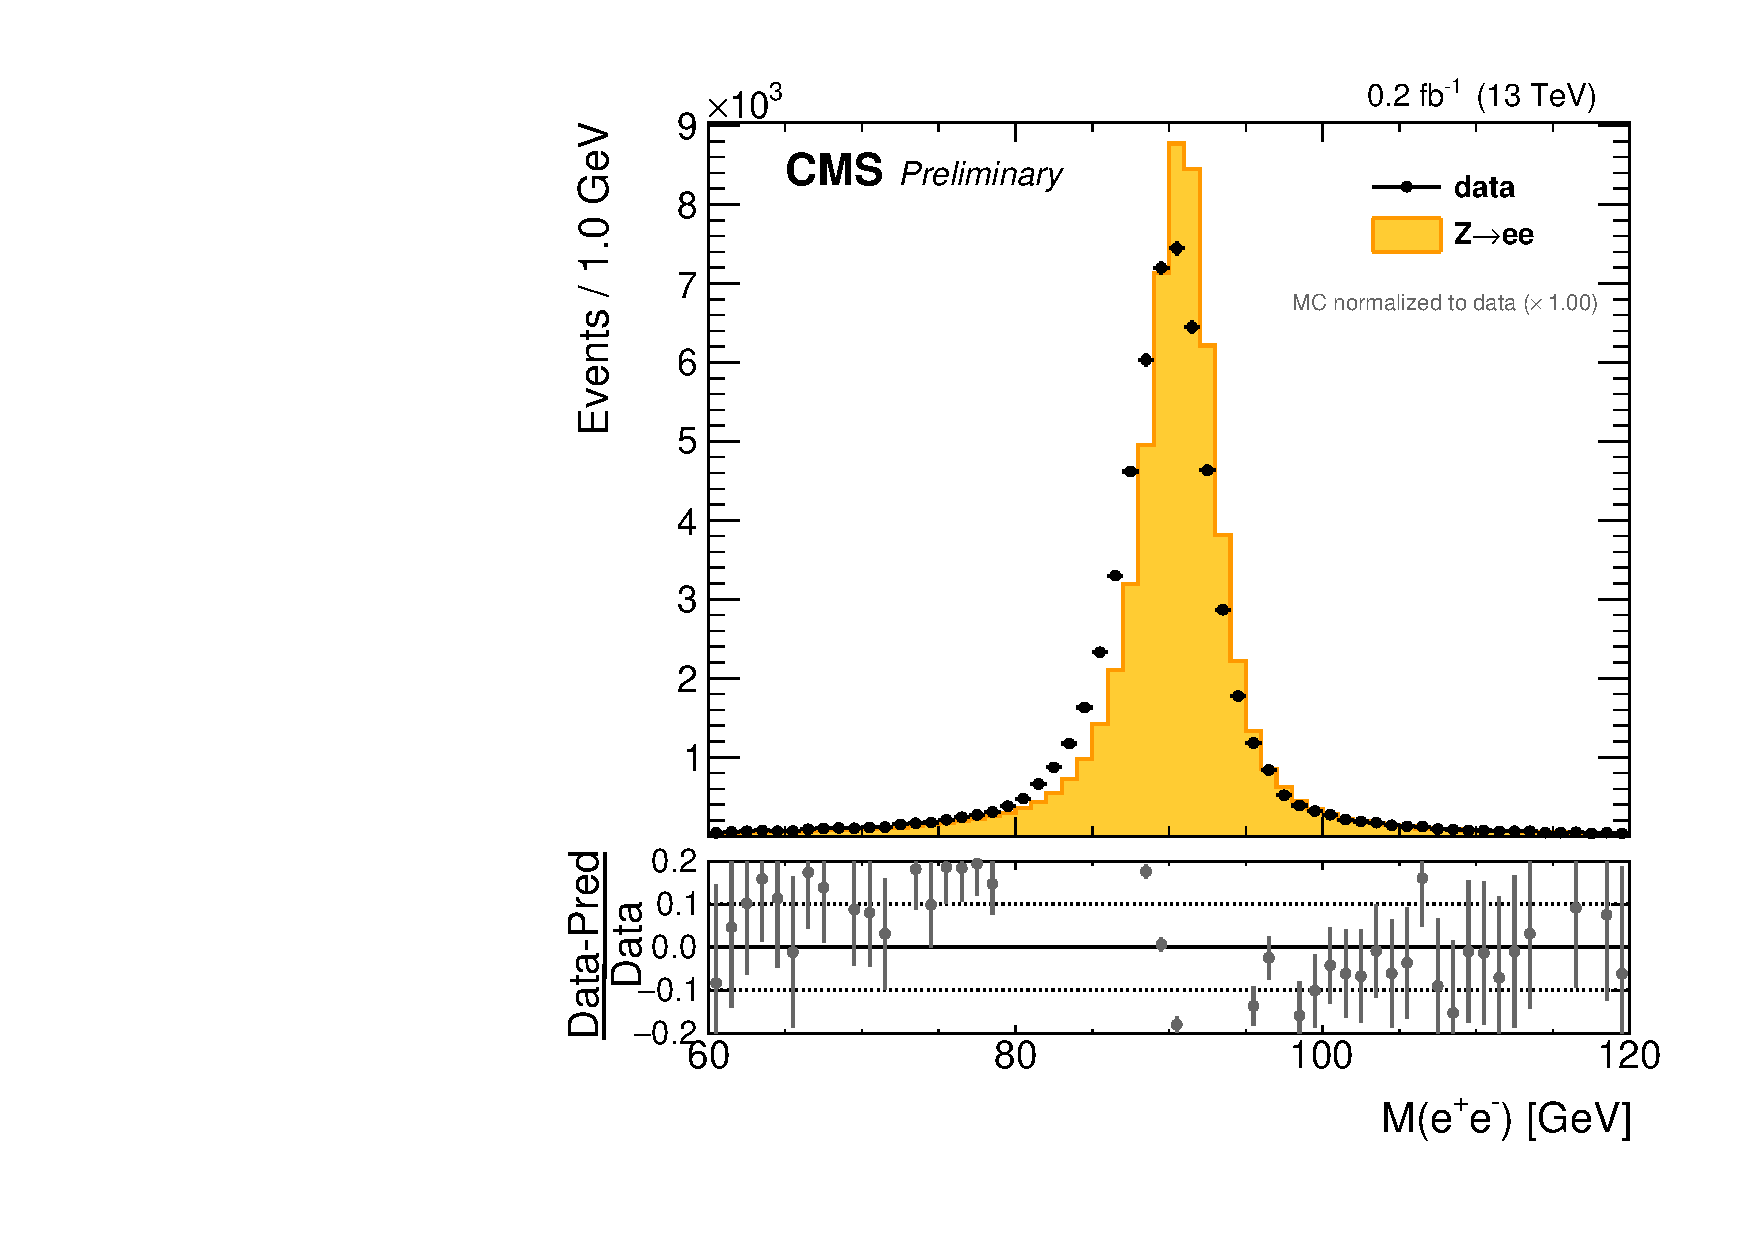
\includegraphics[width=0.49\textwidth]{plots/LepScaleSmear/plotZee13TeV_noCorr/zee_norm.pdf}
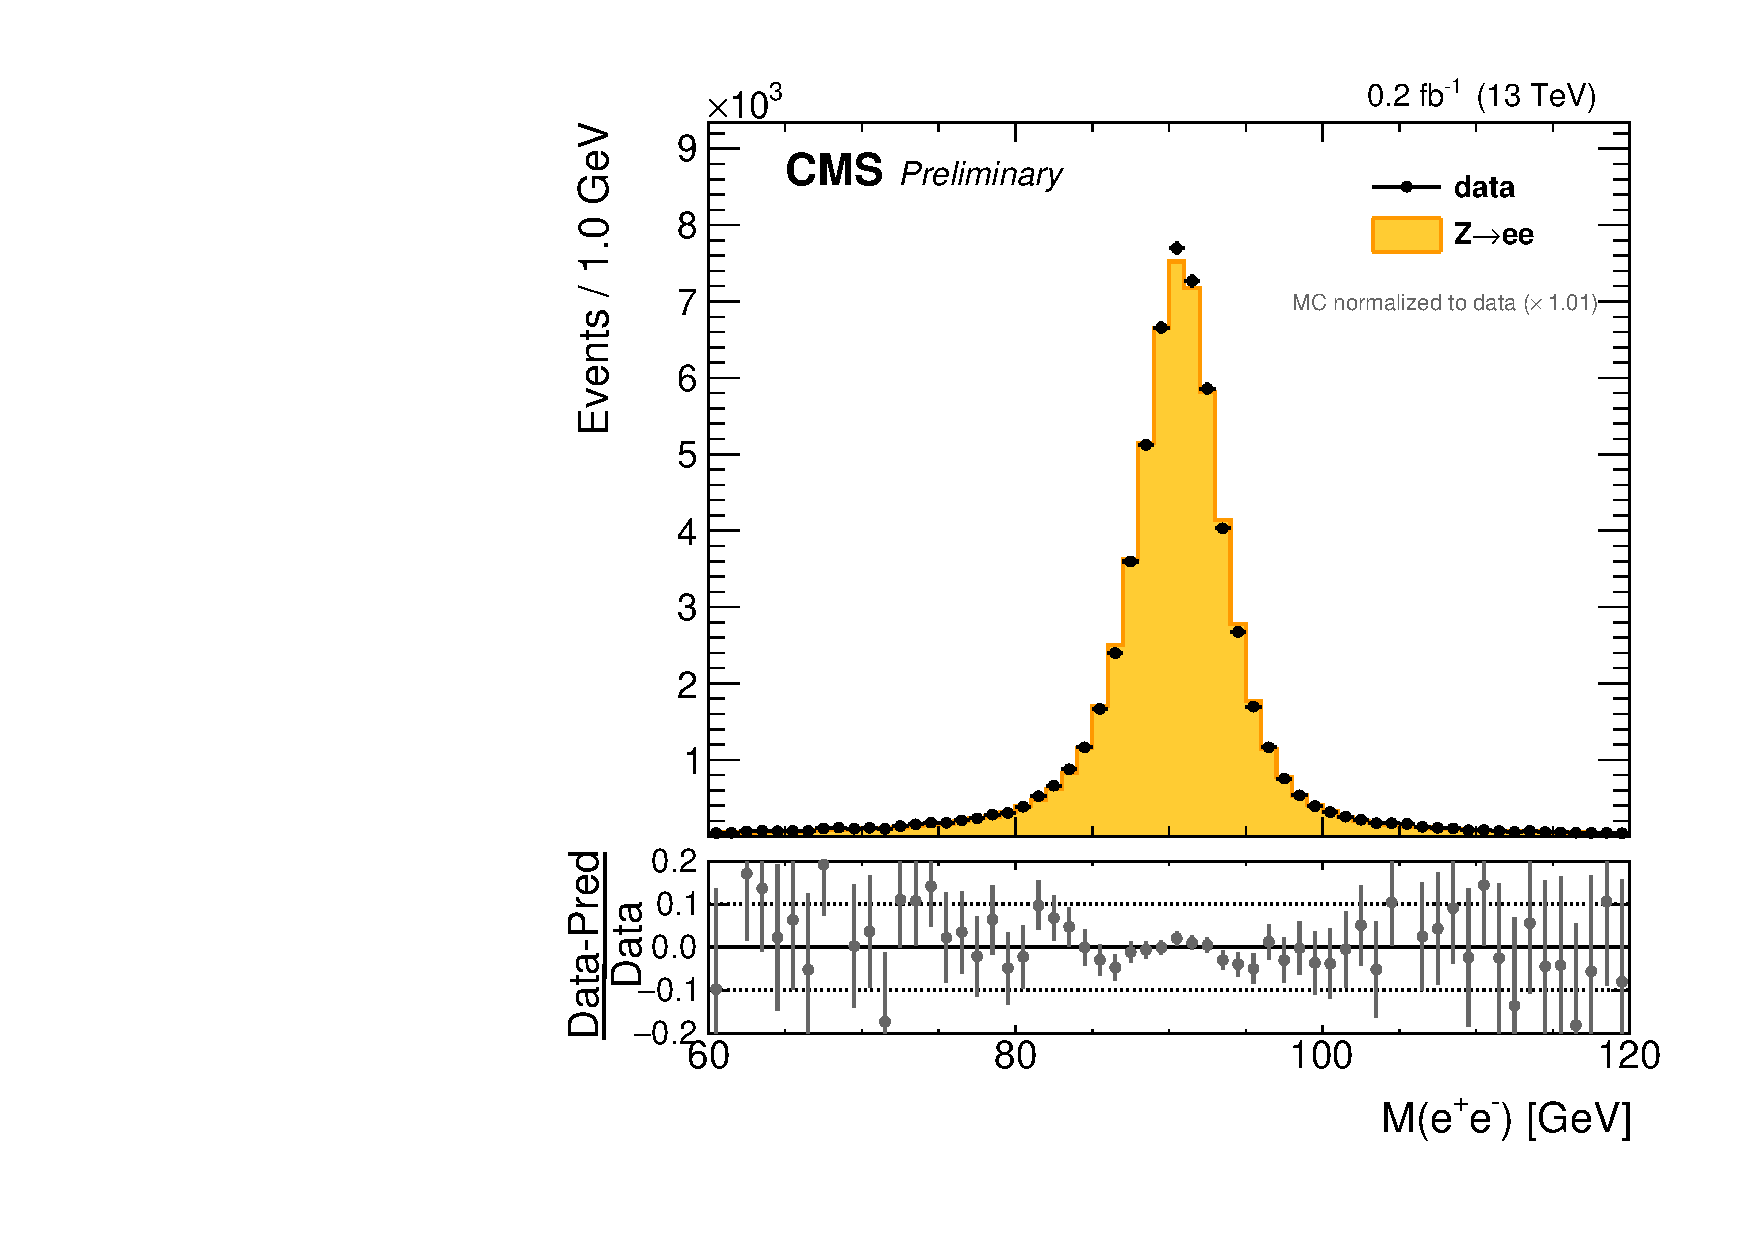
\includegraphics[width=0.49\textwidth]{plots/LepScaleSmear/plotZee13TeV_corr/zee_norm.pdf}
\\
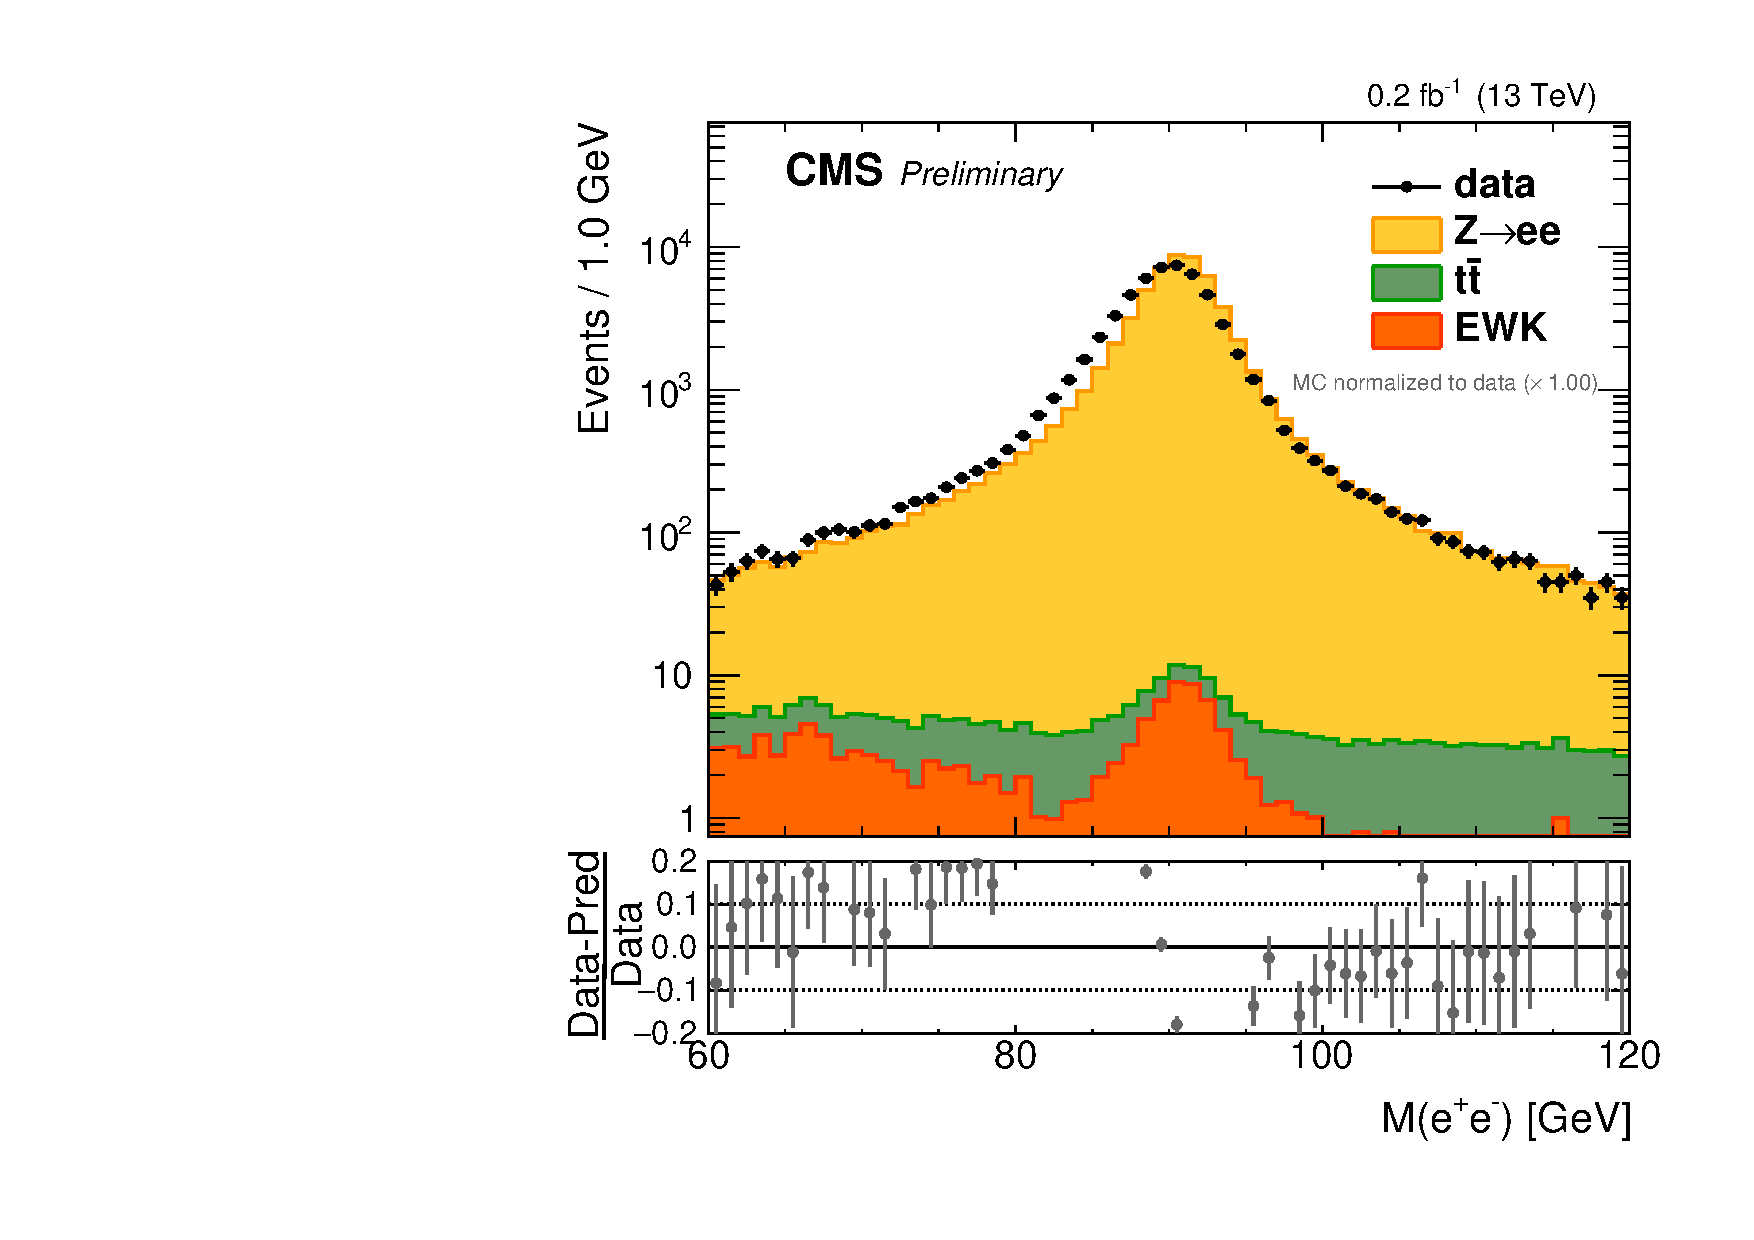
\includegraphics[width=0.49\textwidth]{plots/LepScaleSmear/plotZee13TeV_noCorr/zeelog_norm.pdf}
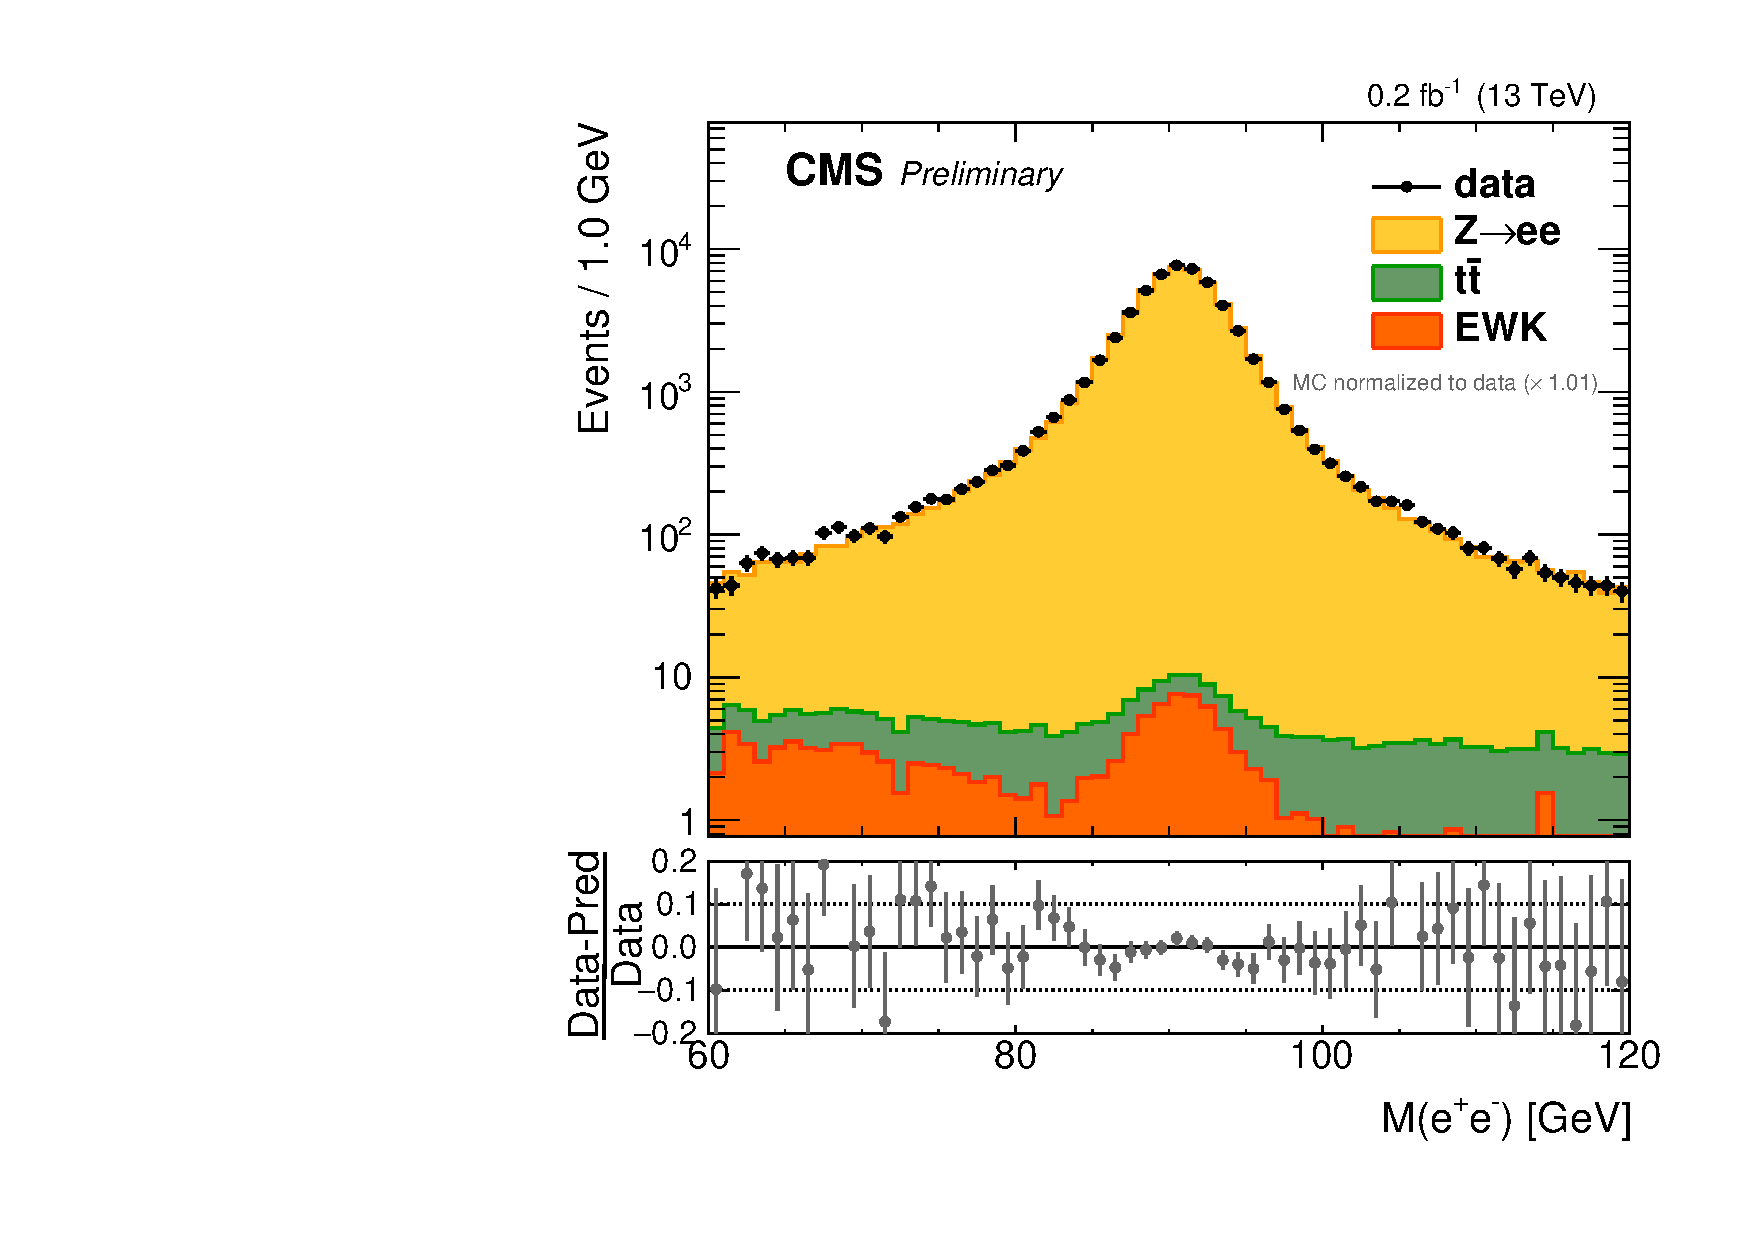
\includegraphics[width=0.49\textwidth]{plots/LepScaleSmear/plotZee13TeV_corr/zeelog_norm.pdf}
\caption{\zee dilepton mass spectrum at \serah, with (right) and without (left) electron energy scale and resolution corrections.}
\label{fig:lepscale:zee:13}
\end{figure}
\begin{figure}[htbp]
\centering
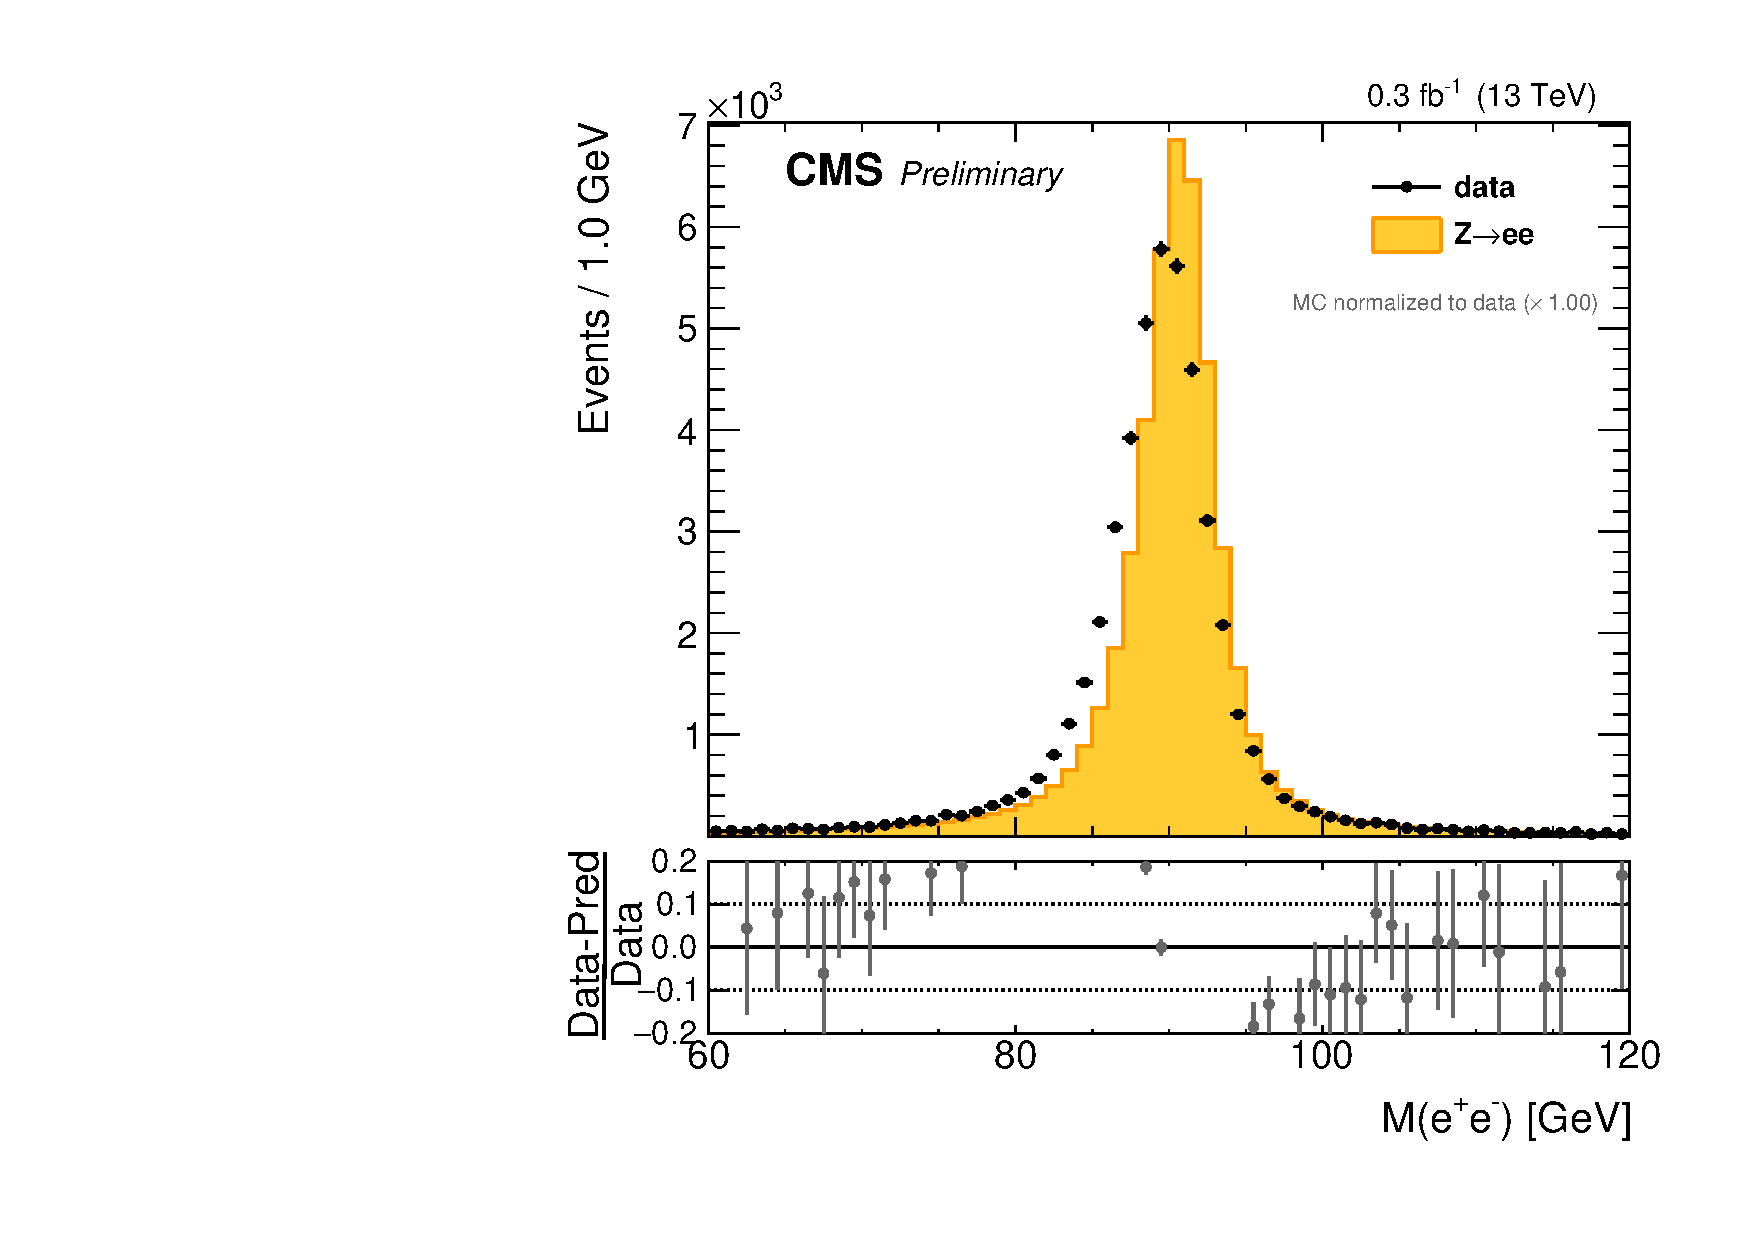
\includegraphics[width=0.49\textwidth]{plots/LepScaleSmear/plotZee5TeV_noCorr/zee_norm.pdf}
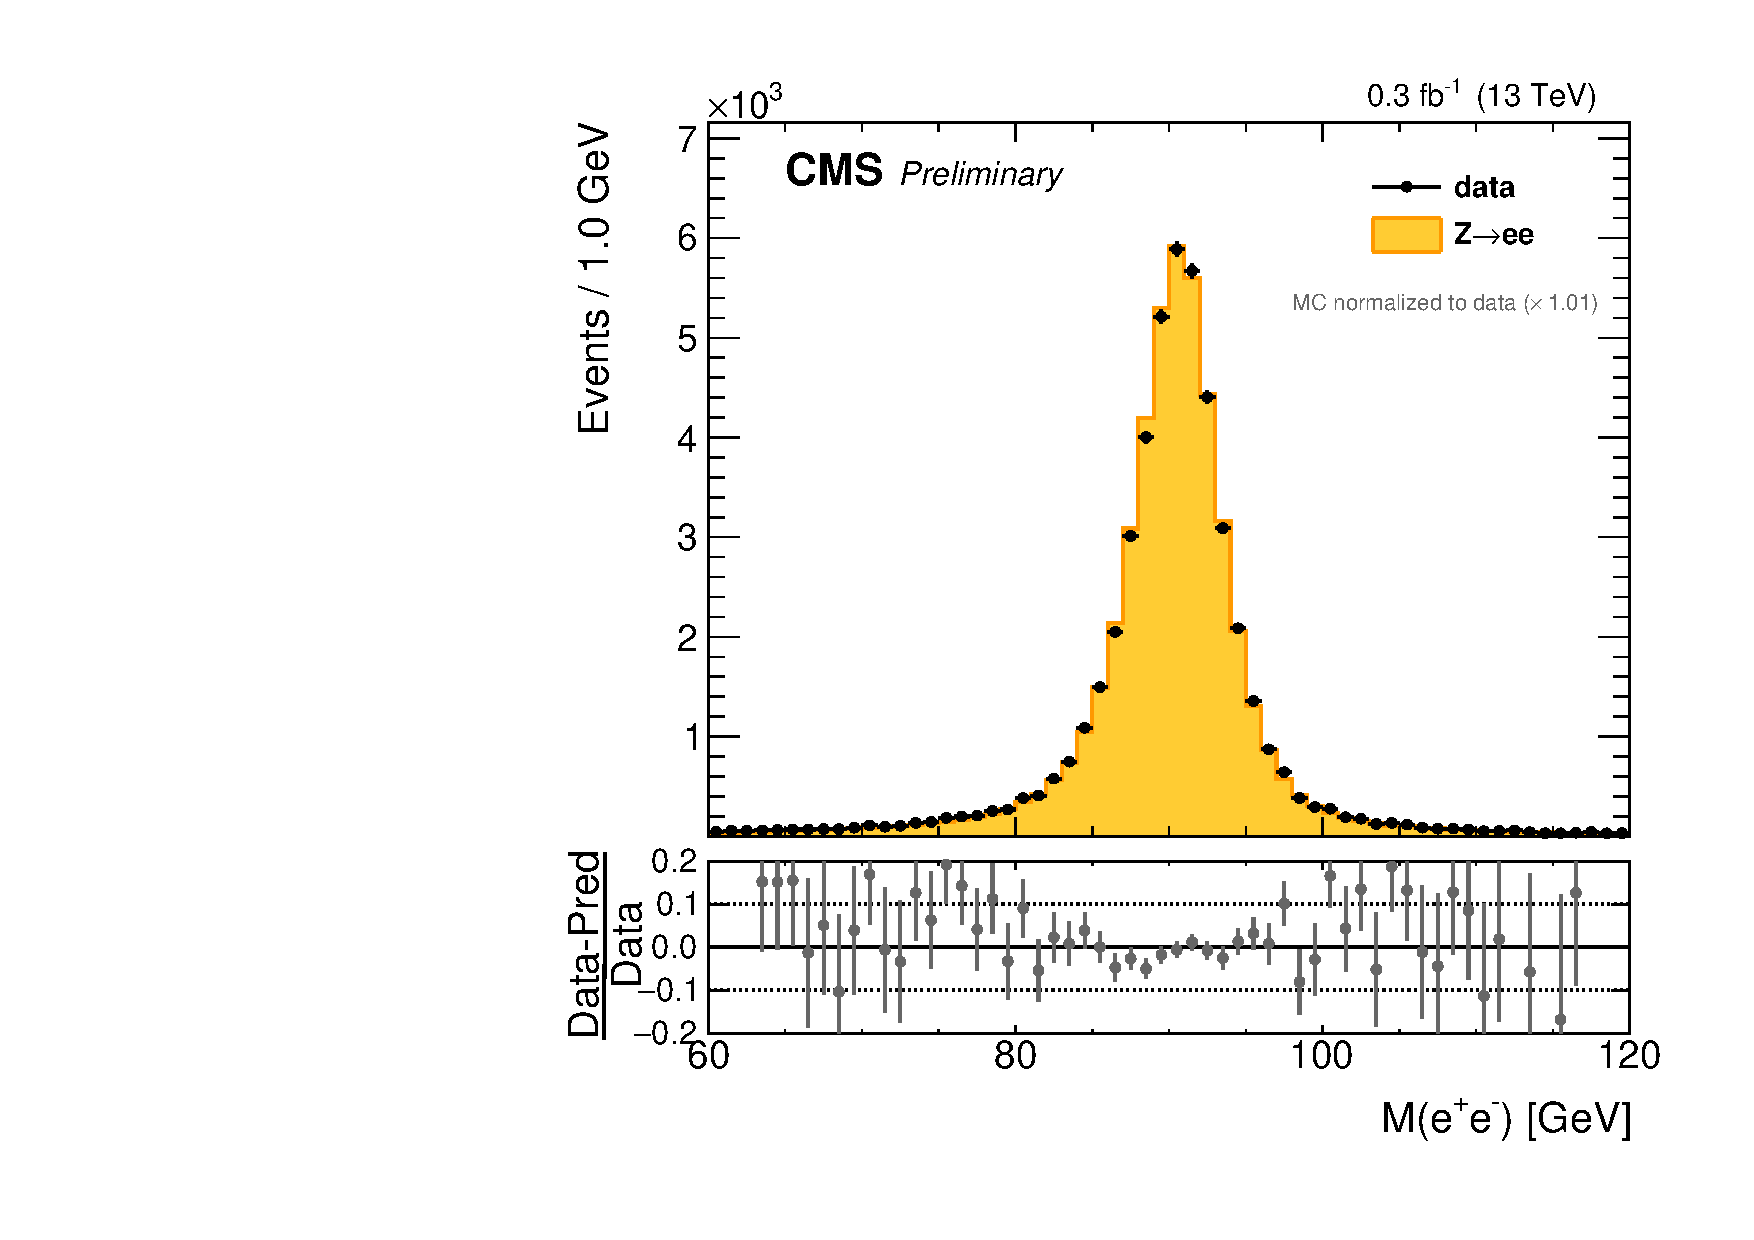
\includegraphics[width=0.49\textwidth]{plots/LepScaleSmear/plotZee5TeV_corr/zee_norm.pdf}
\\
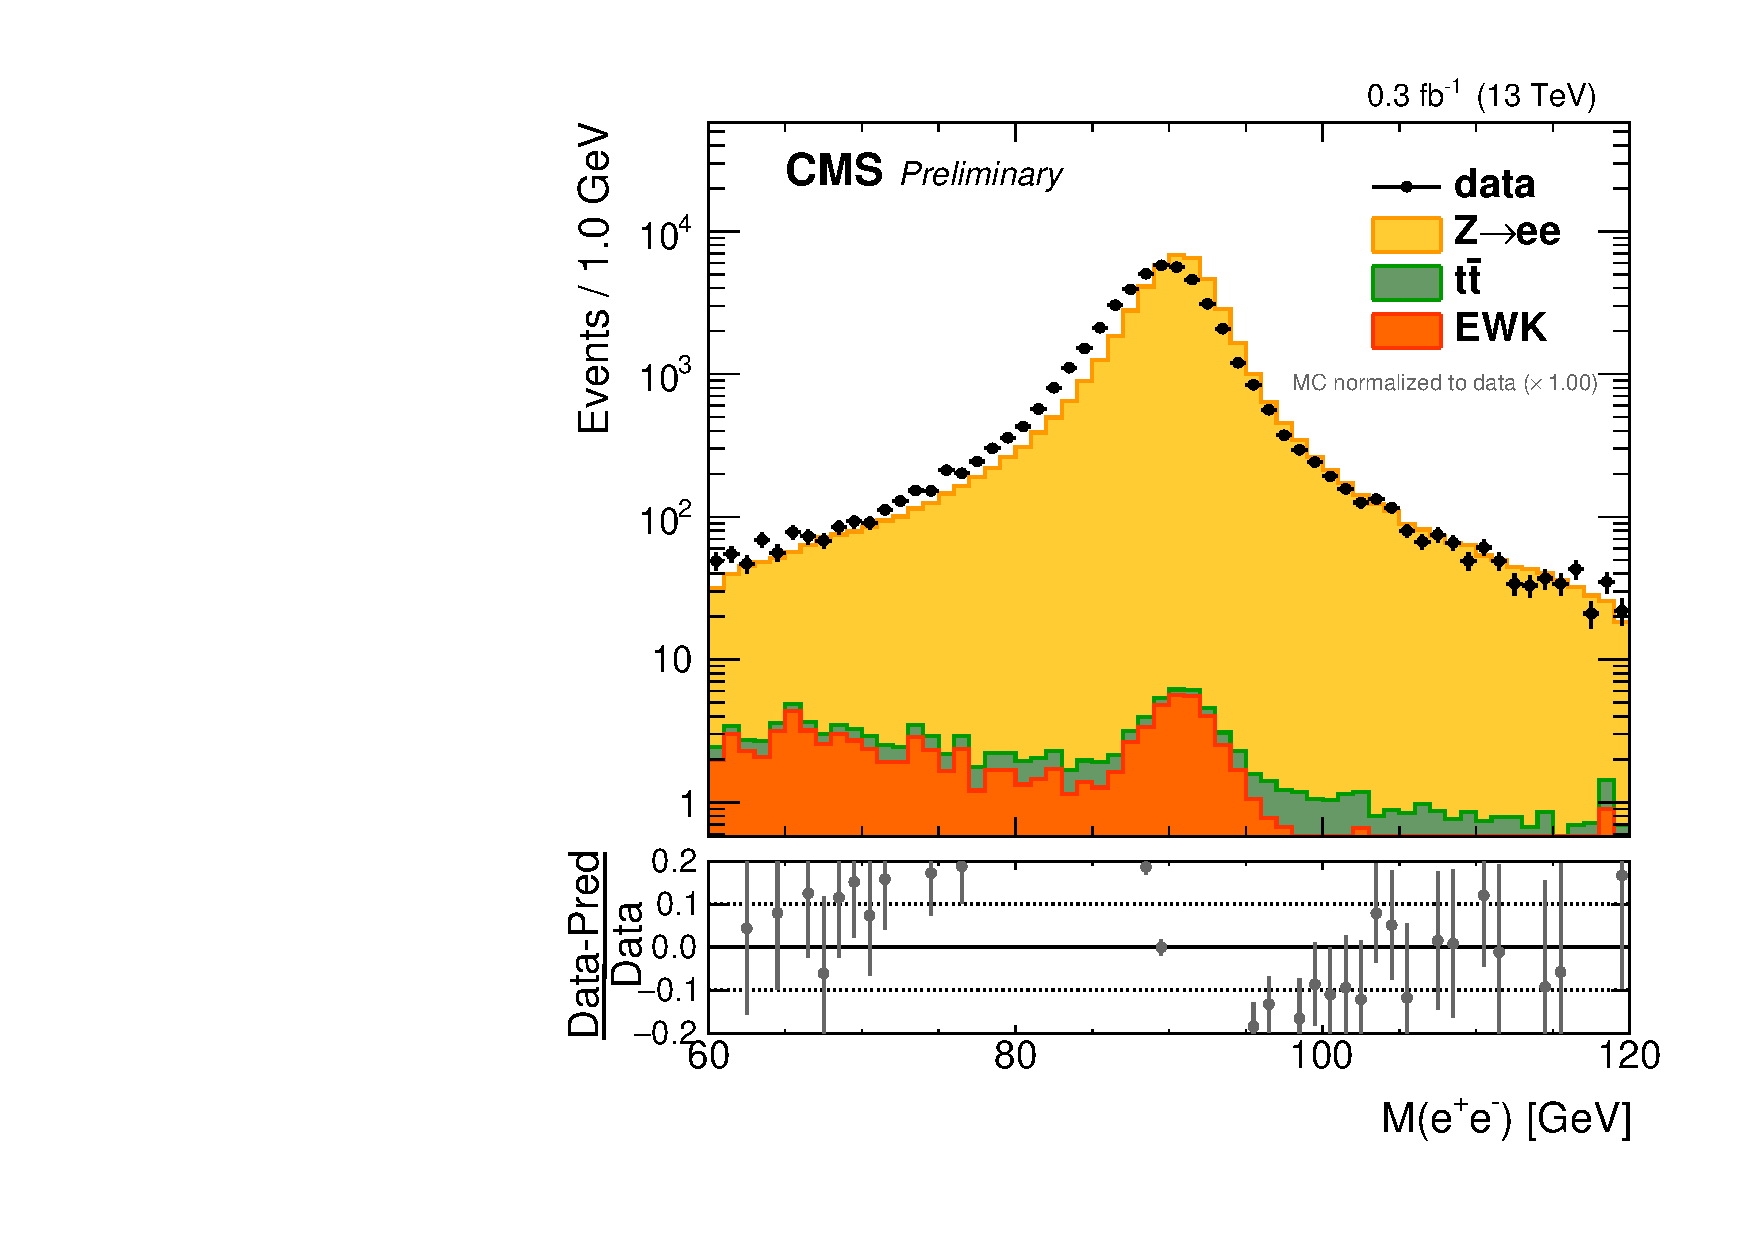
\includegraphics[width=0.49\textwidth]{plots/LepScaleSmear/plotZee5TeV_noCorr/zeelog_norm.pdf}
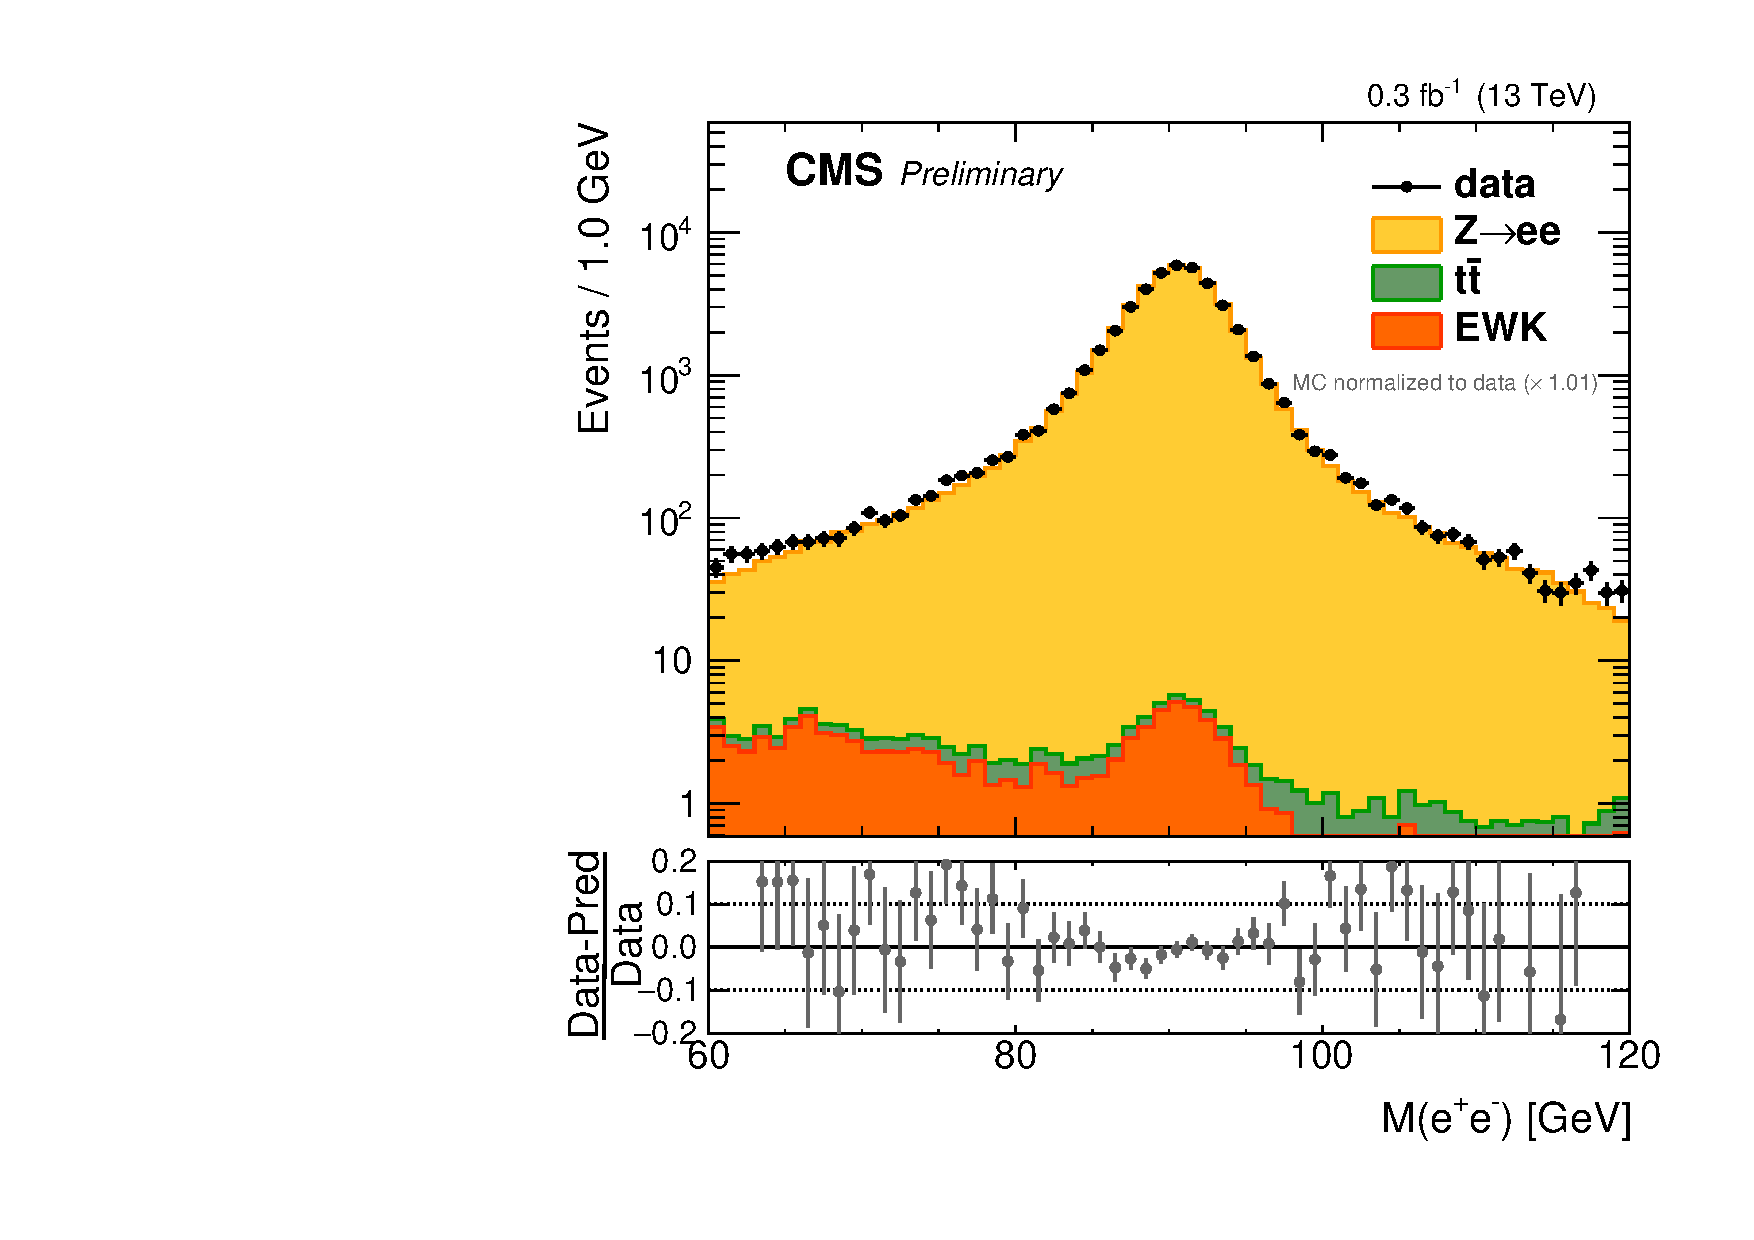
\includegraphics[width=0.49\textwidth]{plots/LepScaleSmear/plotZee5TeV_corr/zeelog_norm.pdf}
\caption{\zee dilepton mass spectrum at \serag, with (right) and without (left) electron energy scale and resolution corrections.}
\label{fig:lepscale:zee:5}
\end{figure}

Scale and resolution corrections for the \serah sample are derived using the method described above, from \zll simulation and the HighEGJet dataset. Scale corrections for data are derived for several sets of run numbers, reflecting changing run conditions and calibrations. Due to statistical limitations, the scale corrections for the \serag data could not be derived in this manner with sufficient $\eta$ granularity. Instead, scale corrections derived for Run 306936 from the \serah data are used along with the smearing corrections derived from the \serah simulation. Run 306936 occurred very shortly after the end of the \serag data taking and the detector conditions are sufficiently similar that these corrections produce adequate results for events from all categories considered.

Systematic uncertainties related to the energy scale and resolution corrections are computed as the difference in \Z boson resonance maximum with variations on energy scale corrections due to selection of electron observables used in correction derivations. 



\subsection{Muon Momentum Corrections}
As with electrons, muon momentum measurements include the need for corrections, though the effect is much smaller than for electrons. Corrections are derived from average lepton \pt and \zmm invariant mass distribution, so that the maximum and width of the \zmm invariant mass in simulation matches data\cite{Bodek:2012id}.  A single set of corrections is used for the entirety of 2017 data-taking. Distributions of \zmm \mll before and after applying muon momentum corrections are shown in Figure~\ref{fig:lepscale:zmm:5} (Figure~\ref{fig:lepscale:zmm:13}) for \serag (\serah).

\begin{figure}[htbp]
\centering
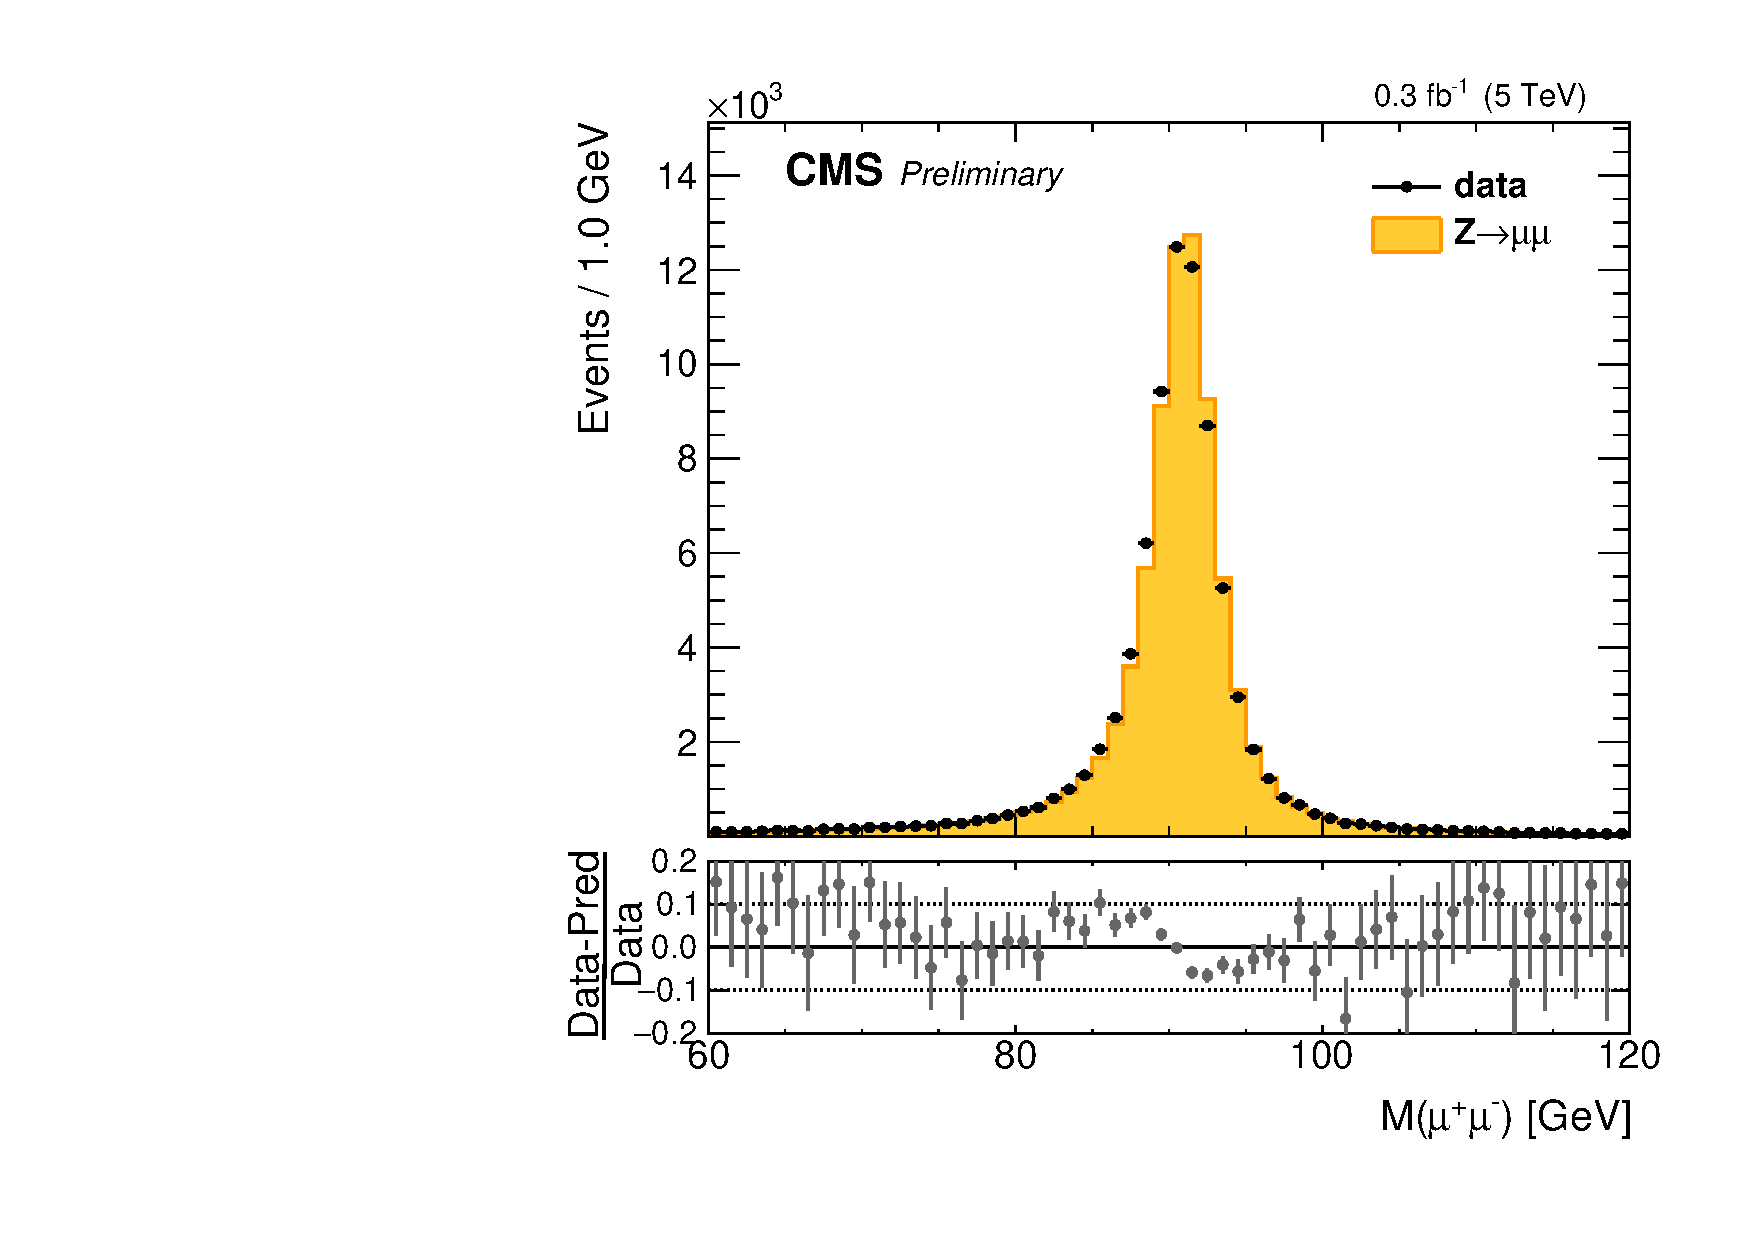
\includegraphics[width=0.49\textwidth]{plots/LepScaleSmear/plotZmm5TeV_noCorr/zmm.pdf}
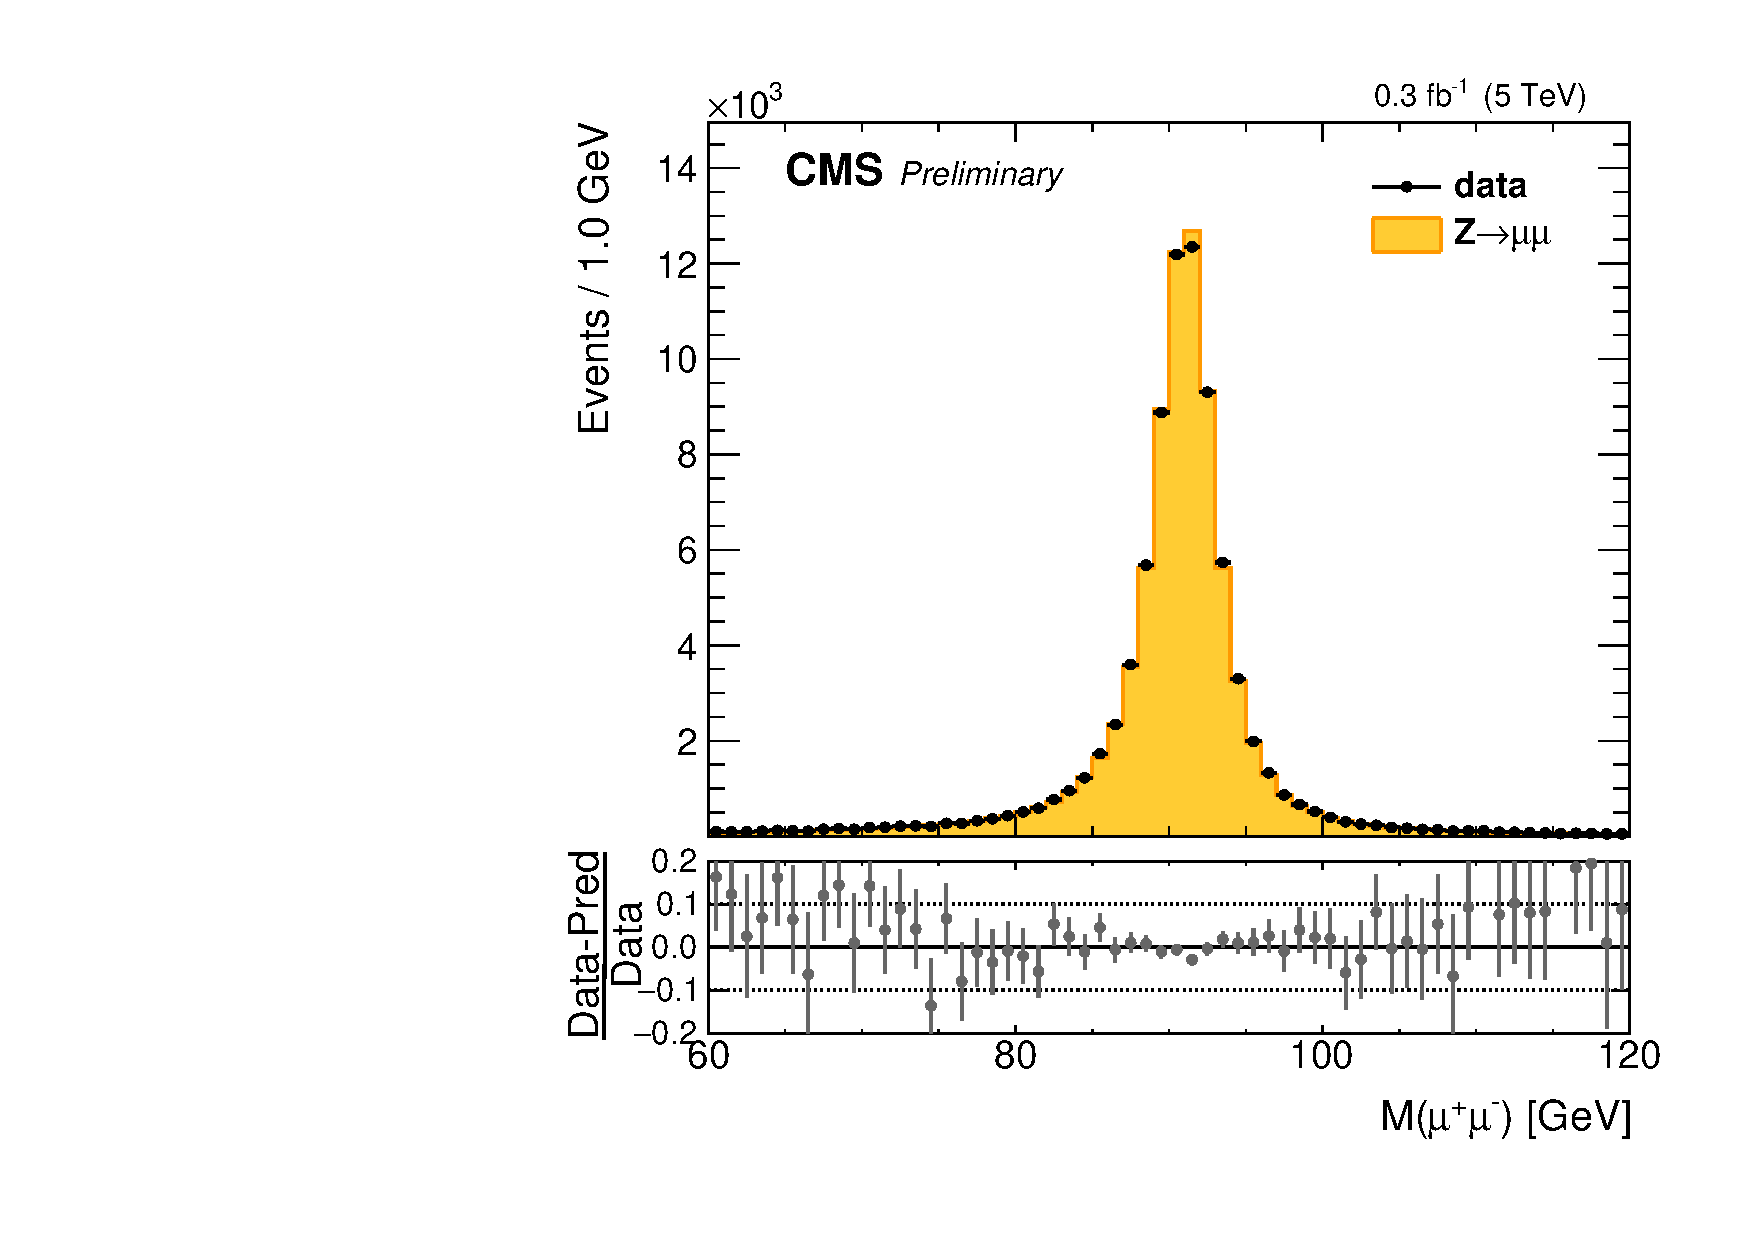
\includegraphics[width=0.49\textwidth]{plots/LepScaleSmear/plotZmm5TeV_corr/zmm.pdf}
\\
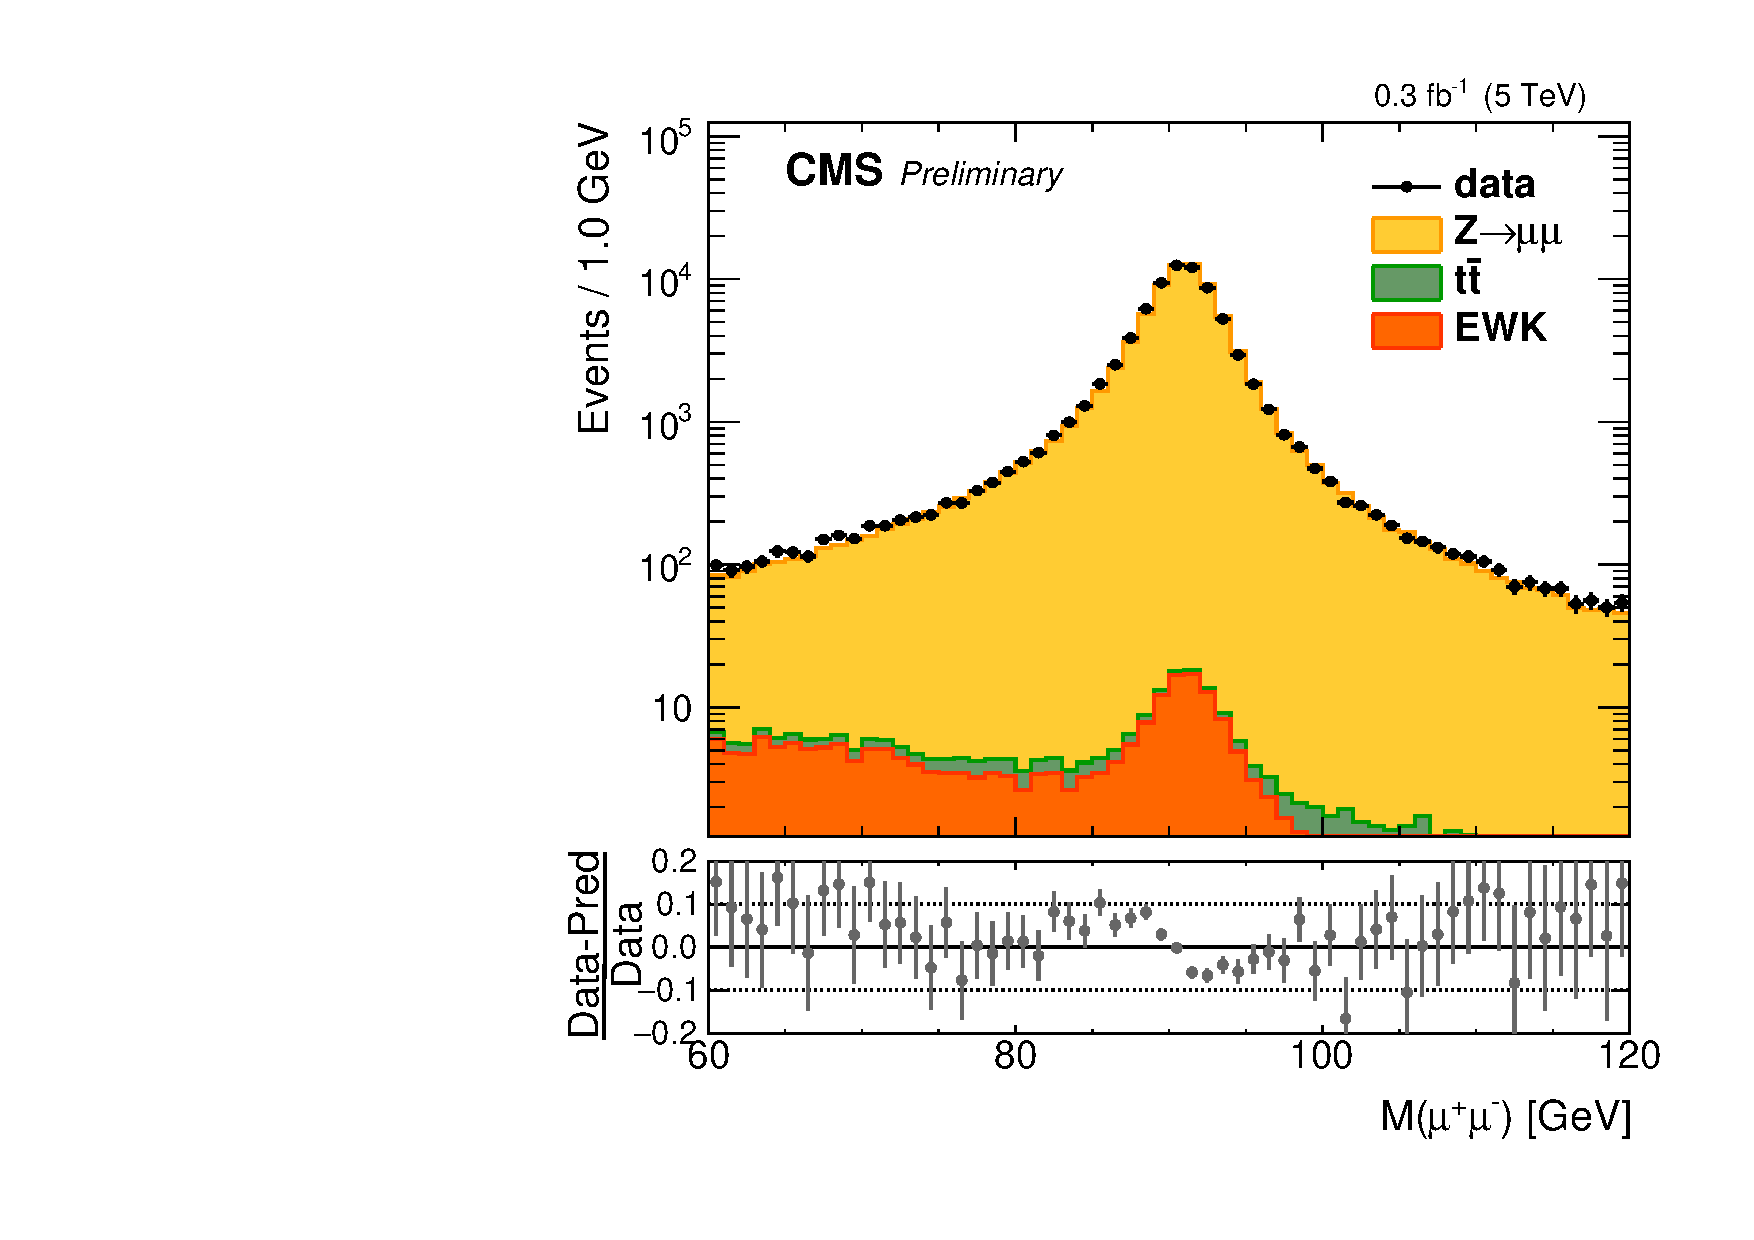
\includegraphics[width=0.49\textwidth]{plots/LepScaleSmear/plotZmm5TeV_noCorr/zmmlog.pdf}
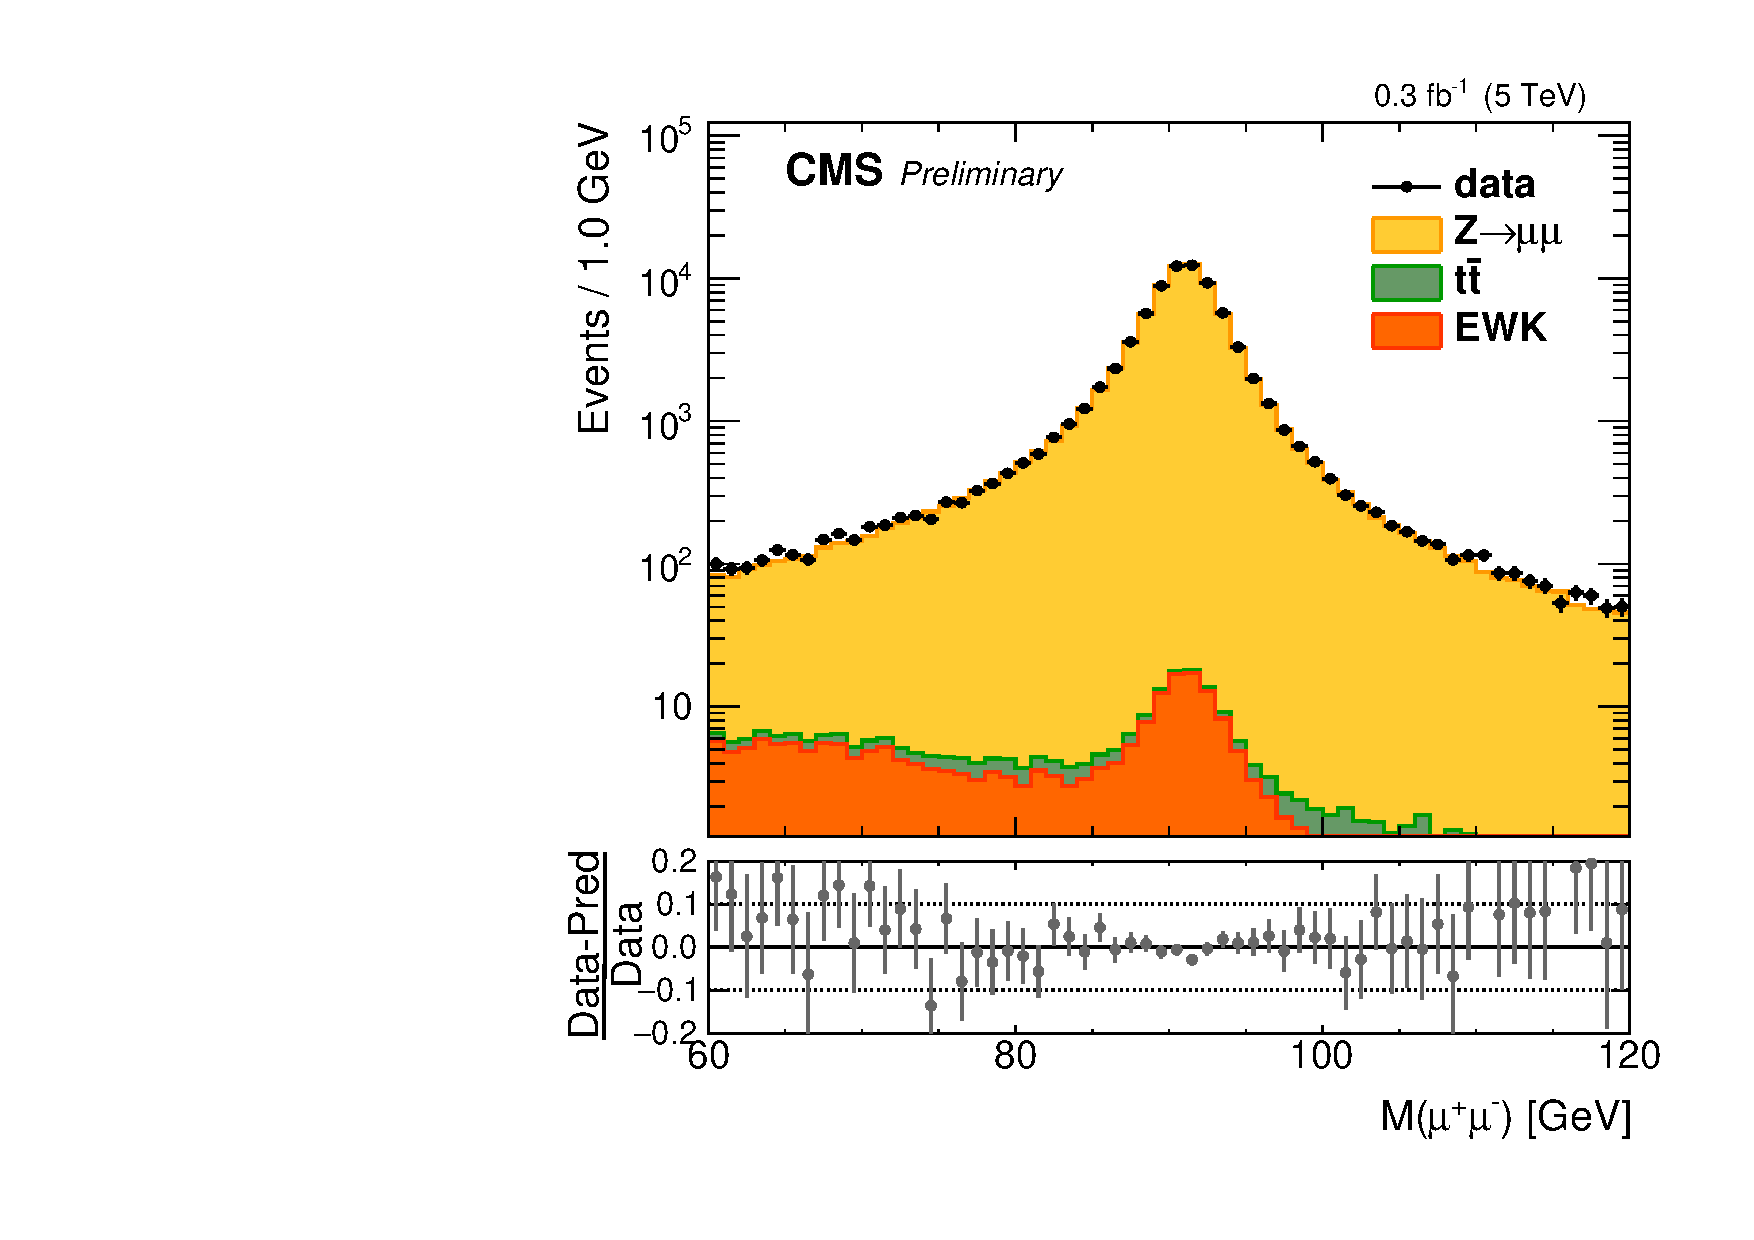
\includegraphics[width=0.49\textwidth]{plots/LepScaleSmear/plotZmm5TeV_corr/zmmlog.pdf}
\caption{\zmm dilepton mass spectrum at \sg, with (right) and without (left) muon Rochester corrections.}
\label{fig:lepscale:zmm:5}
\end{figure}
\begin{figure}[htbp]
\centering
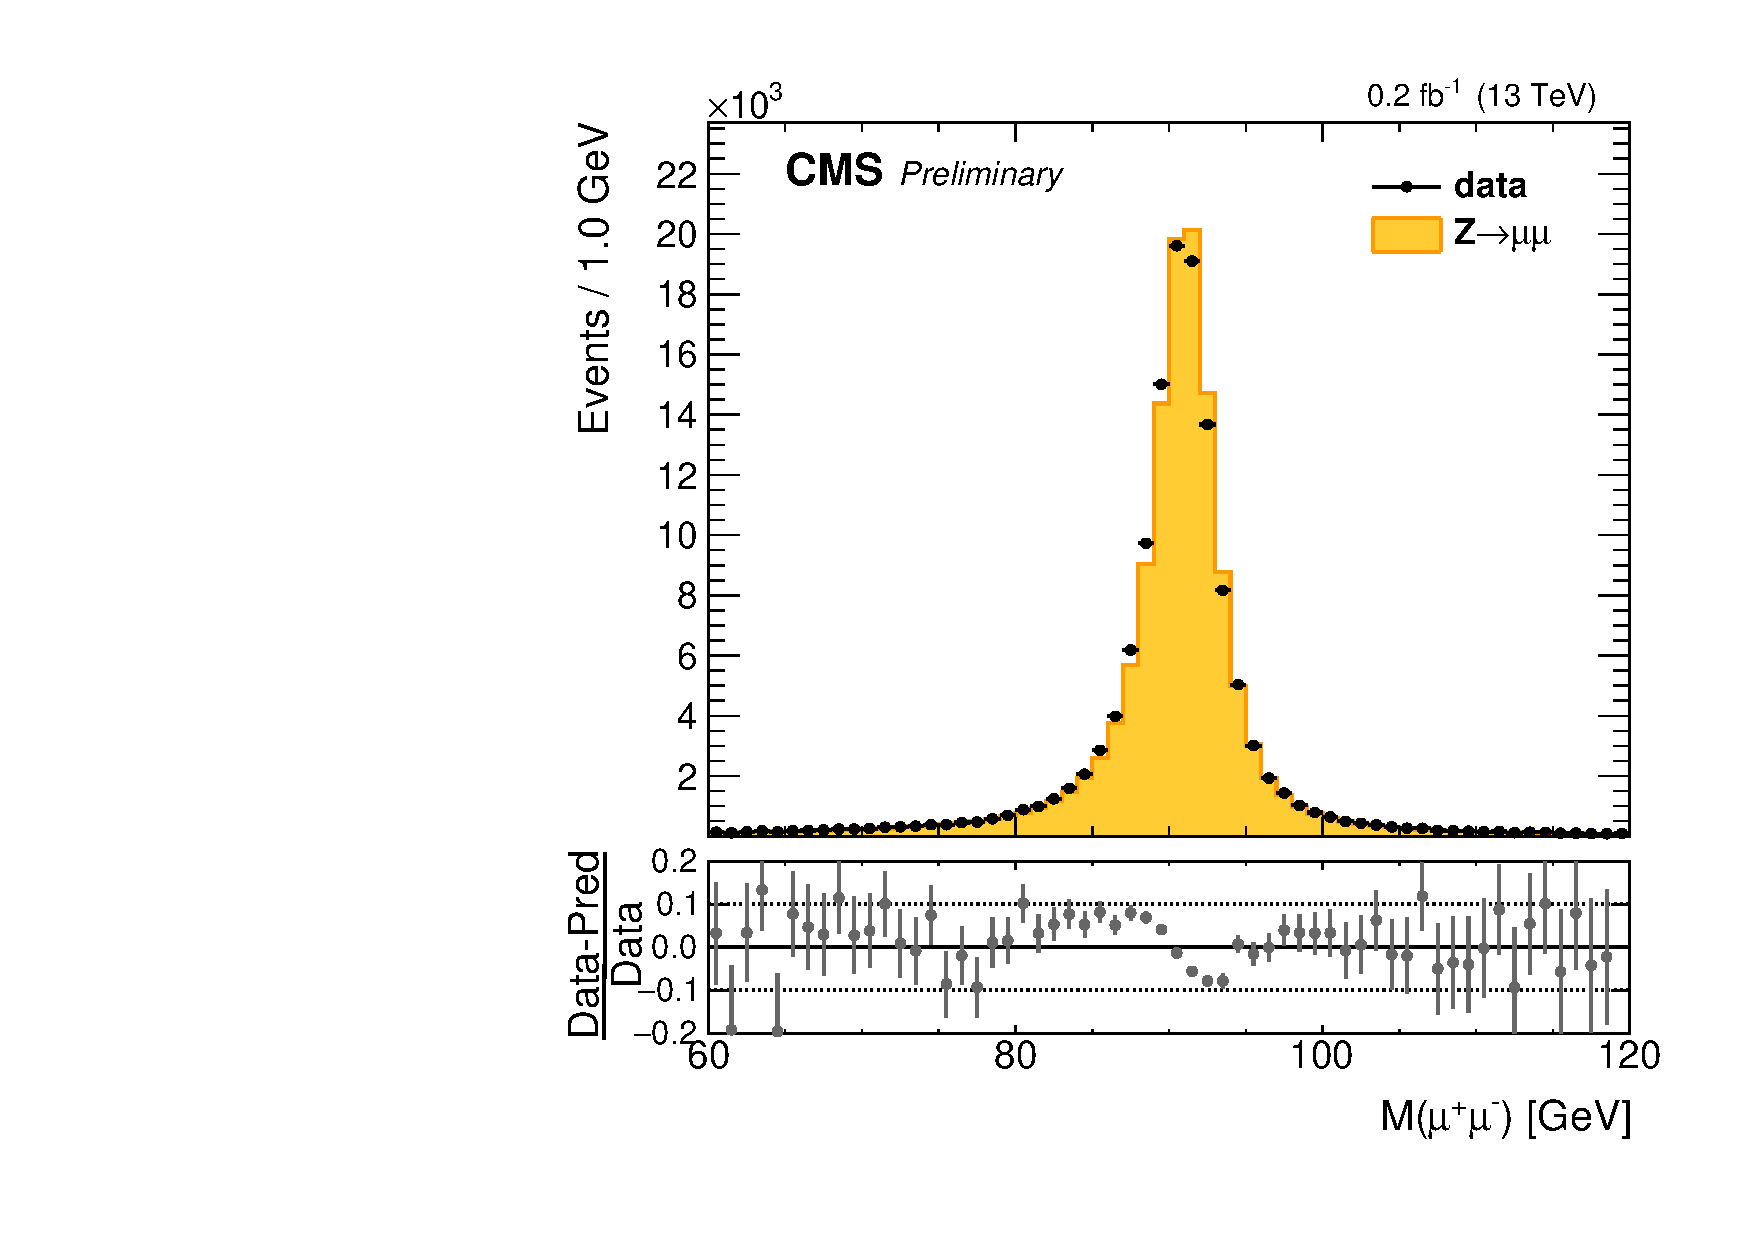
\includegraphics[width=0.49\textwidth]{plots/LepScaleSmear/plotZmm13TeV_noCorr/zmm.pdf}
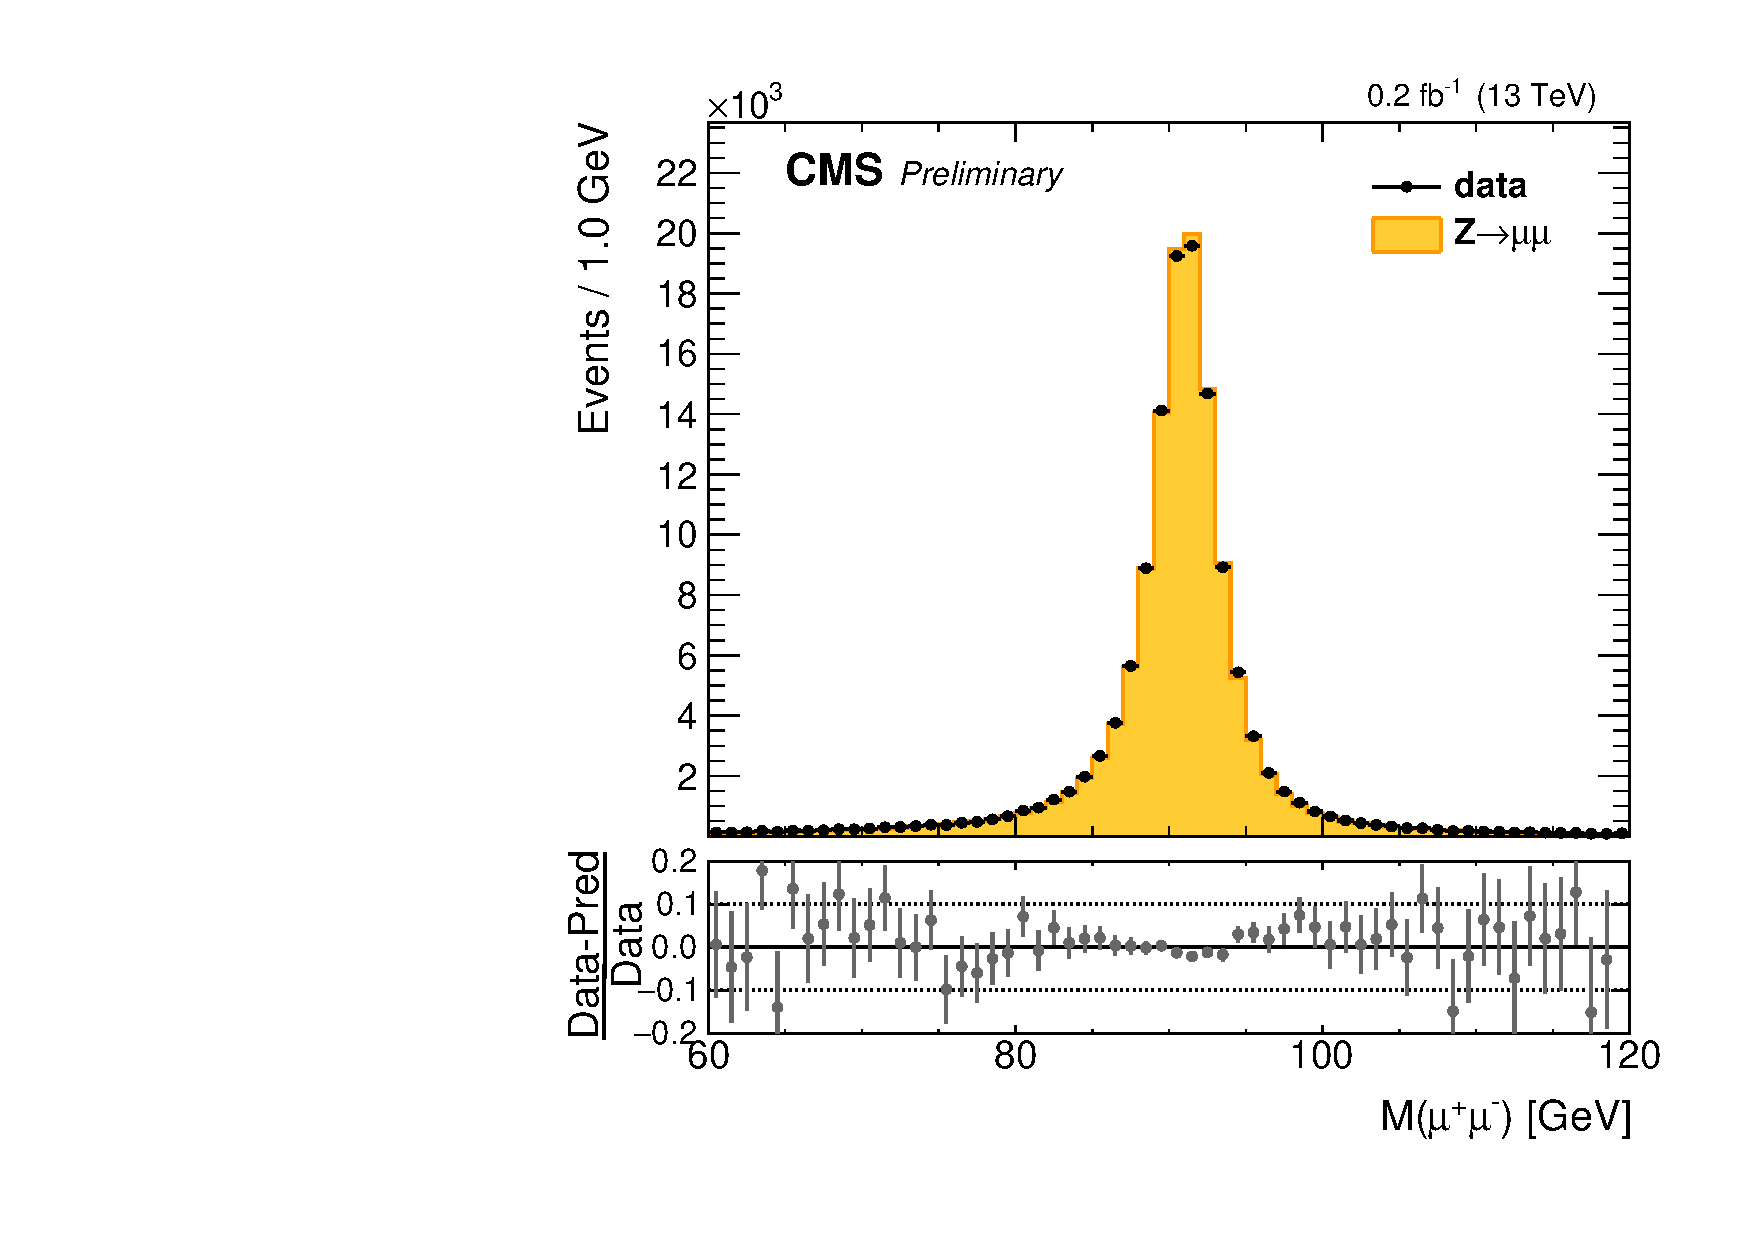
\includegraphics[width=0.49\textwidth]{plots/LepScaleSmear/plotZmm13TeV_corr/zmm.pdf}
\\
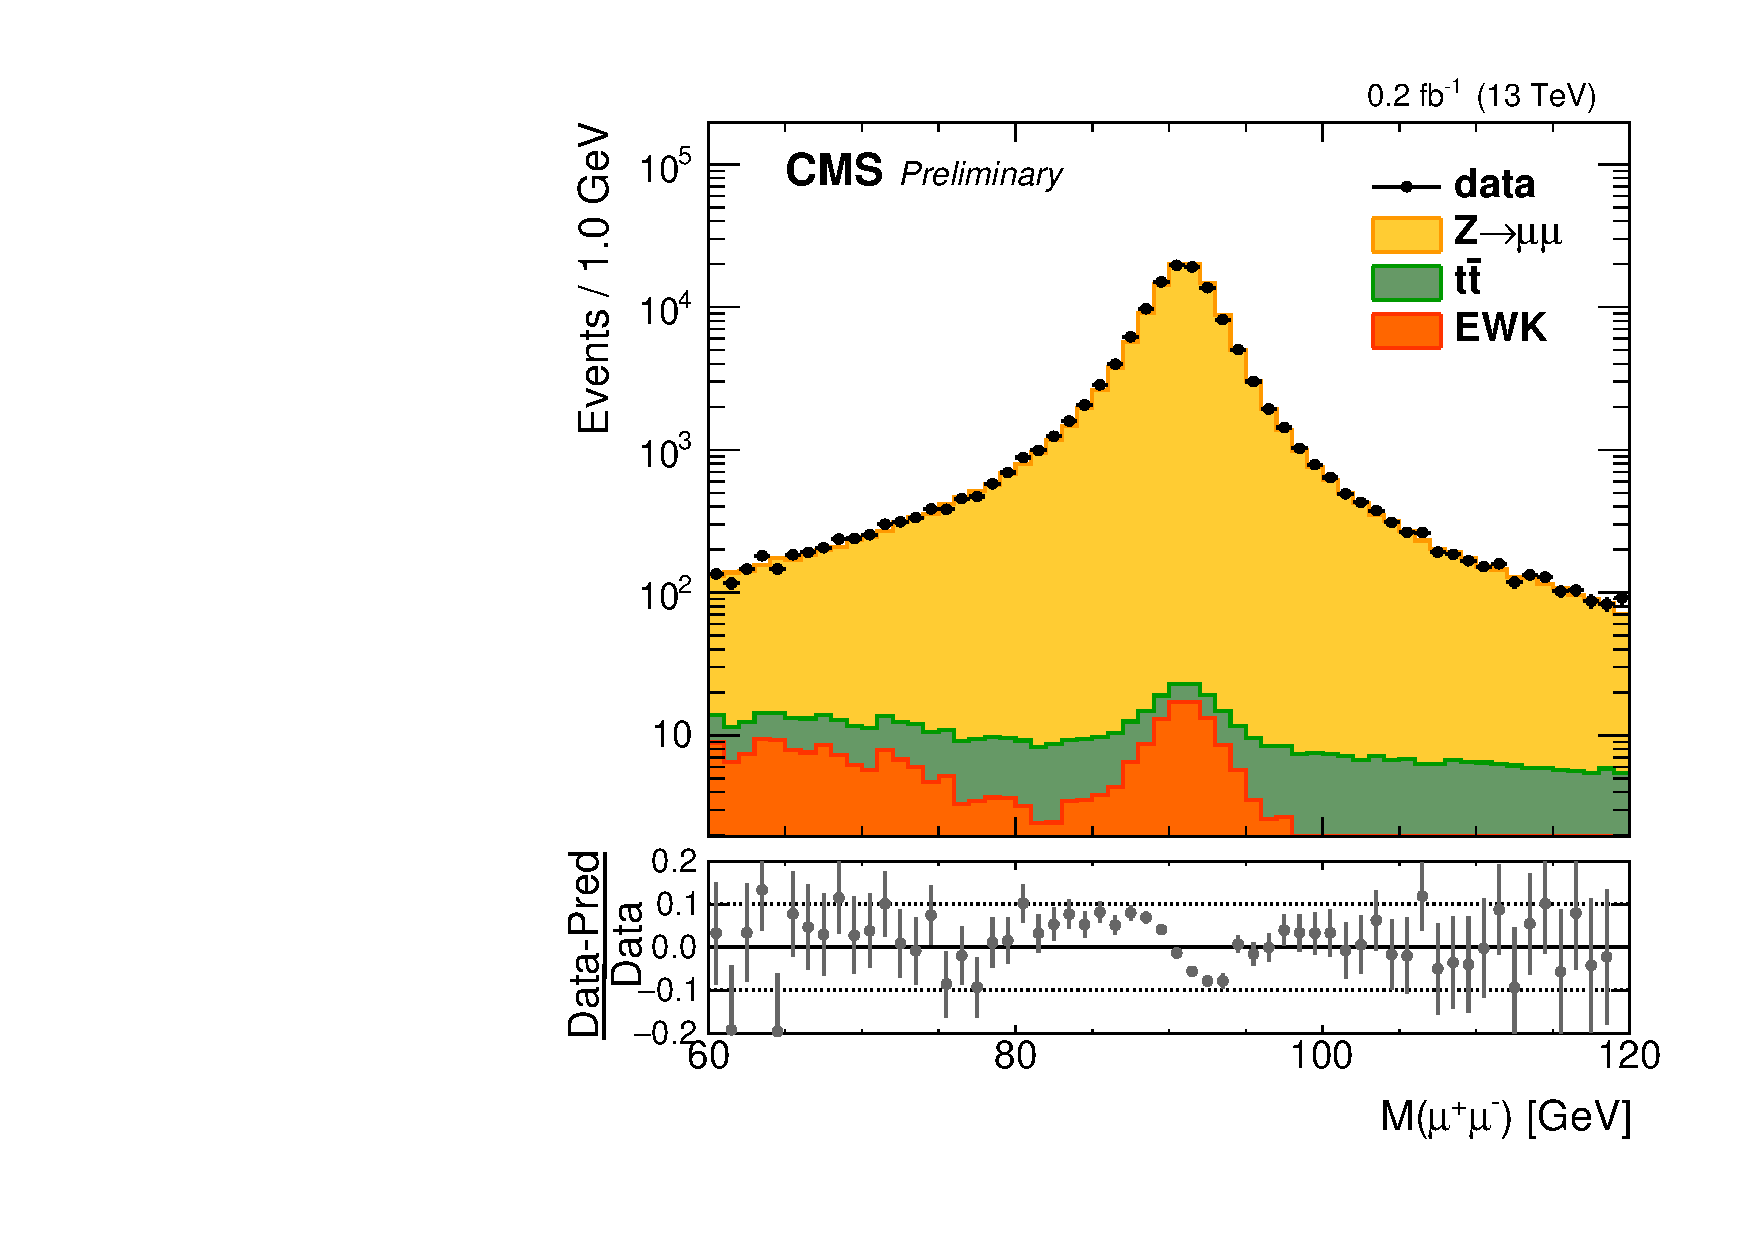
\includegraphics[width=0.49\textwidth]{plots/LepScaleSmear/plotZmm13TeV_noCorr/zmmlog.pdf}
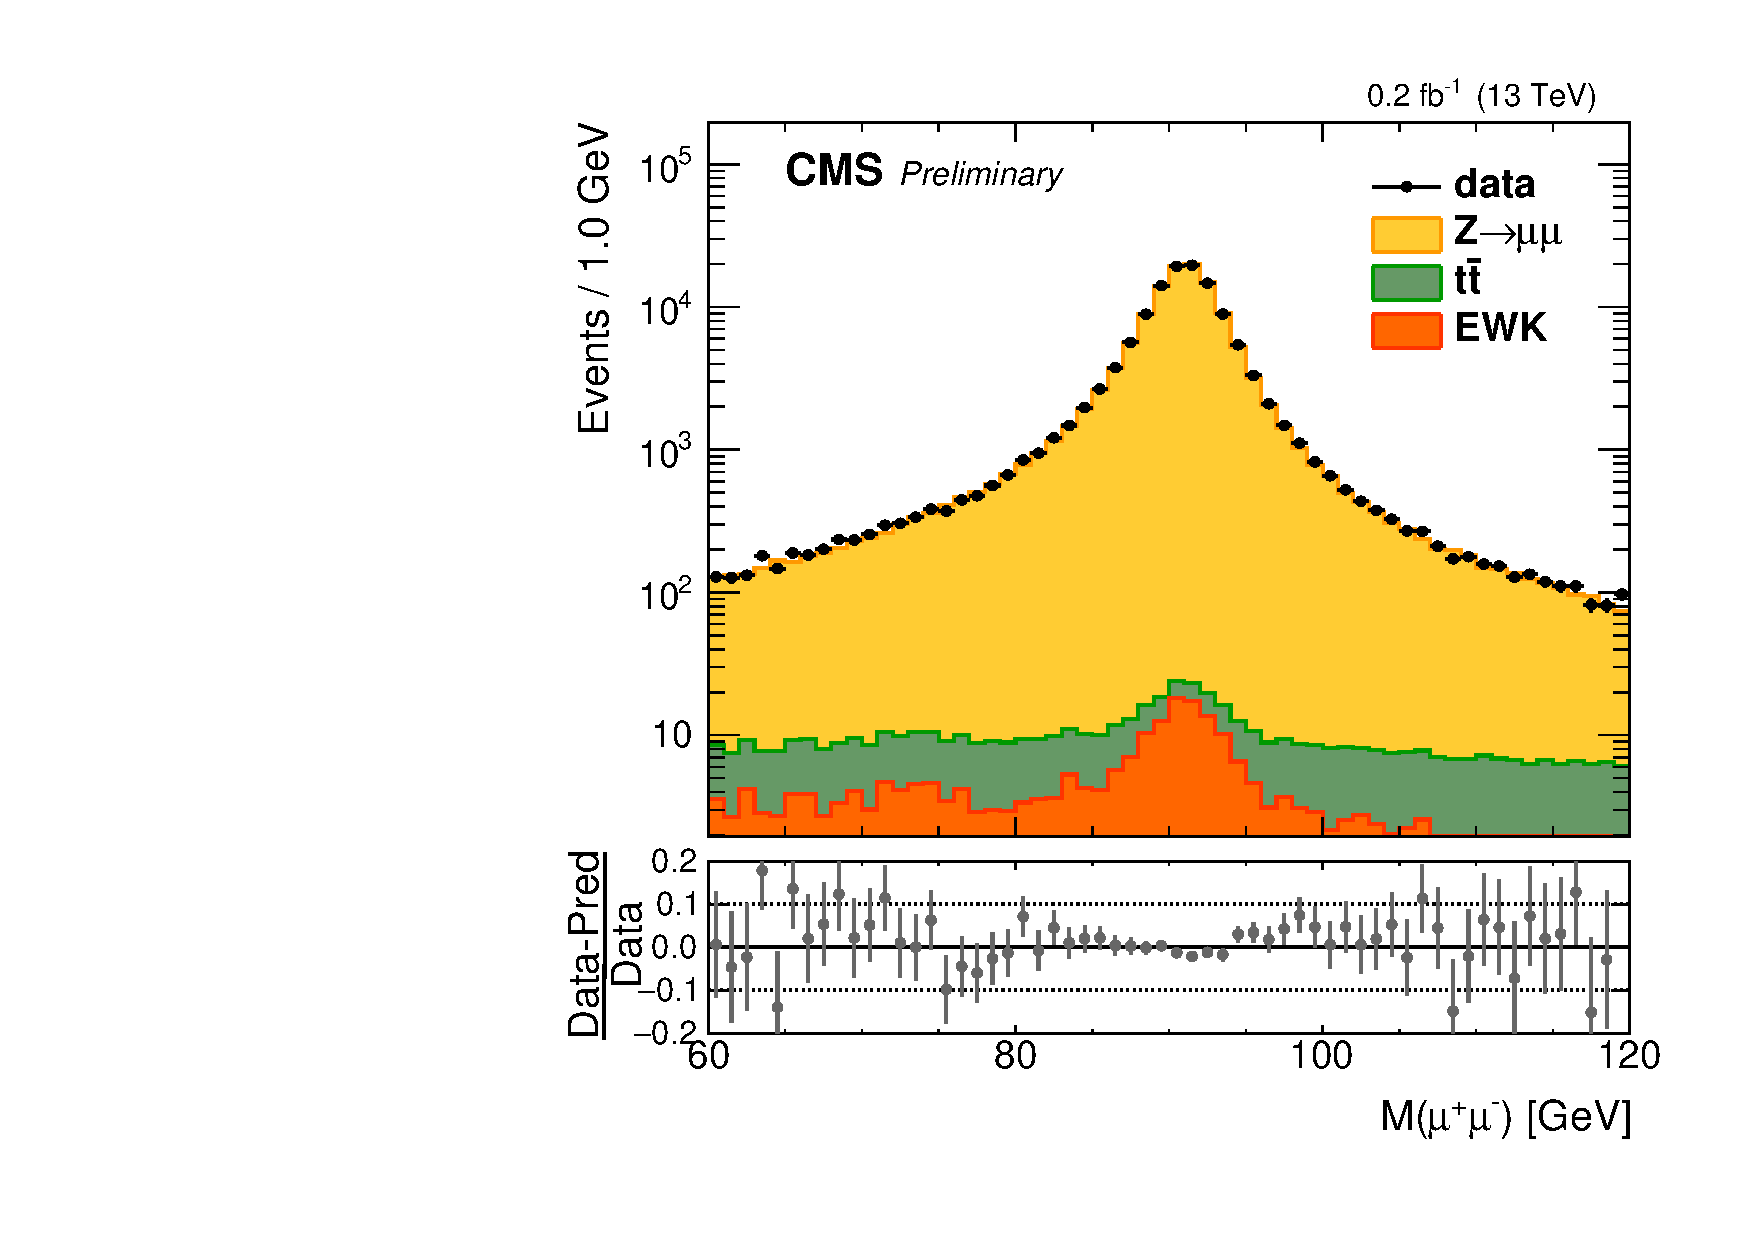
\includegraphics[width=0.49\textwidth]{plots/LepScaleSmear/plotZmm13TeV_corr/zmmlog.pdf}
\caption{\zmm dilepton mass spectrum at \sh, with (right) and without (left) muon momentum corrections.}
\label{fig:lepscale:zmm:13}
\end{figure}


%%%%%%%%%%%%%%%%%%%%%%%%%%%%%%%%%%%%%%%%%%%%
%                Prefiring

\section{ECAL L1 Trigger Prefiring}\label{ch:prefire}
Radiation damage to the PbWO4 crystals in the ECAL result in color centers forming within the crystal lattice, reducing transparency and altering light propagation through the crystal. Corrections to accommodate the change in scintillation light transmission were not applied in a way which completely removed the timing drift. Trigger primitives (TPs) in the forward regions of ECAL, $2.0 < |\eta| < 3.5$, were affected by the timing drift during the 2017 data-taking period. The timing drift caused certain TPs in the forward ECAL region to be incorrectly associated with the wrong bunch crossing, an effect described as "pre-firing". The global trigger rules disallow the collection of consecutive bunch crossings, so an event which contains a pre-fired trigger primitive will cause the BX-1 (previous bunch crossing) to be read out, while BX0 (the current one containing the actual event with the TP) to be discarded by the trigger. In all likelihood, the read out event will not pass the HLT and will ultimately be discarded.
This effect is not described in simulation, but a correction factor describing the rate of event loss is derived from data. A pre-firing probability is assigned to each simulated event, based on the kinematics of the photons and jets present in the event, in Equation~\ref{eq:prefiring_weight}, re-scales contribution of simulated events given the likelihood of pre-firing.
\begin{figure}[htbp]
\centering
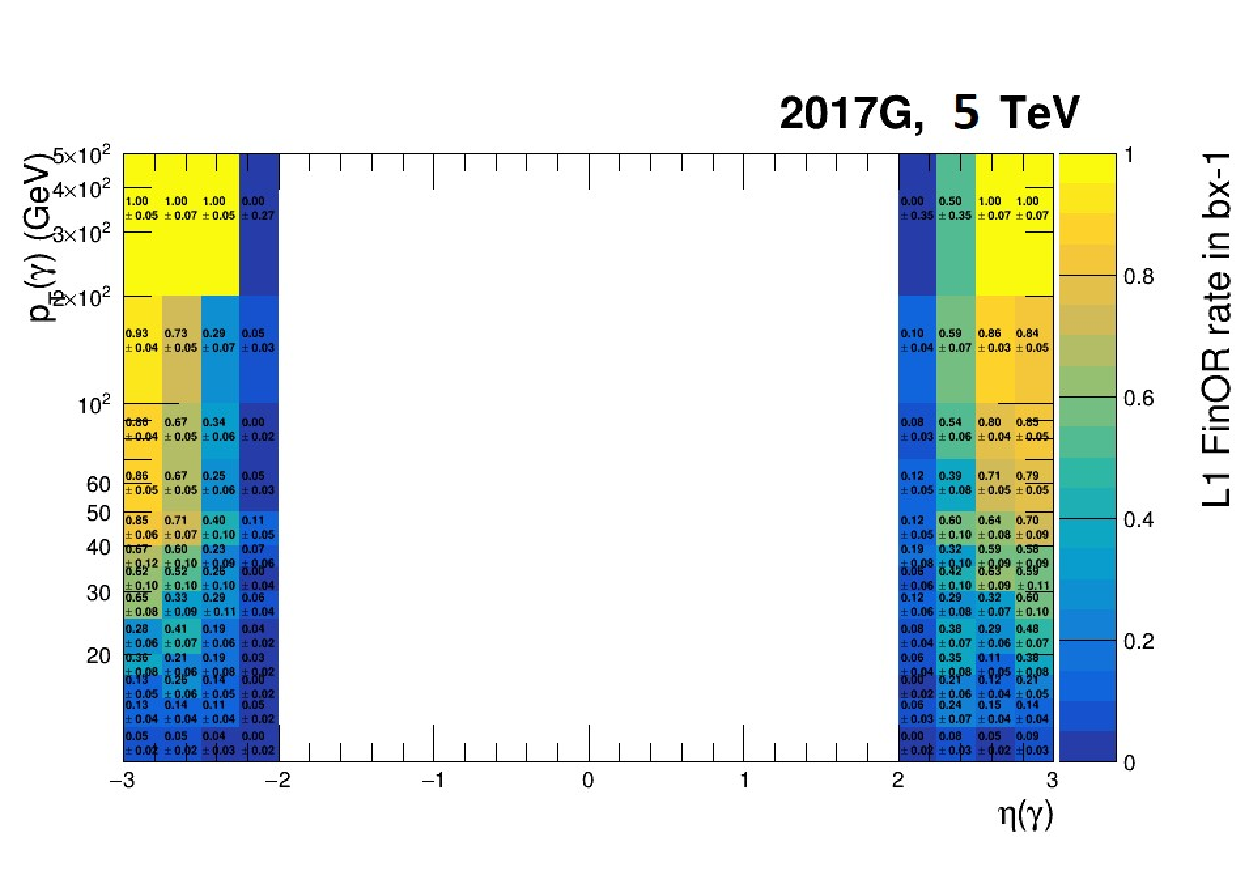
\includegraphics[width=0.49\textwidth]{plots/Prefire/L1prefiring_photonpt_2017G.pdf}
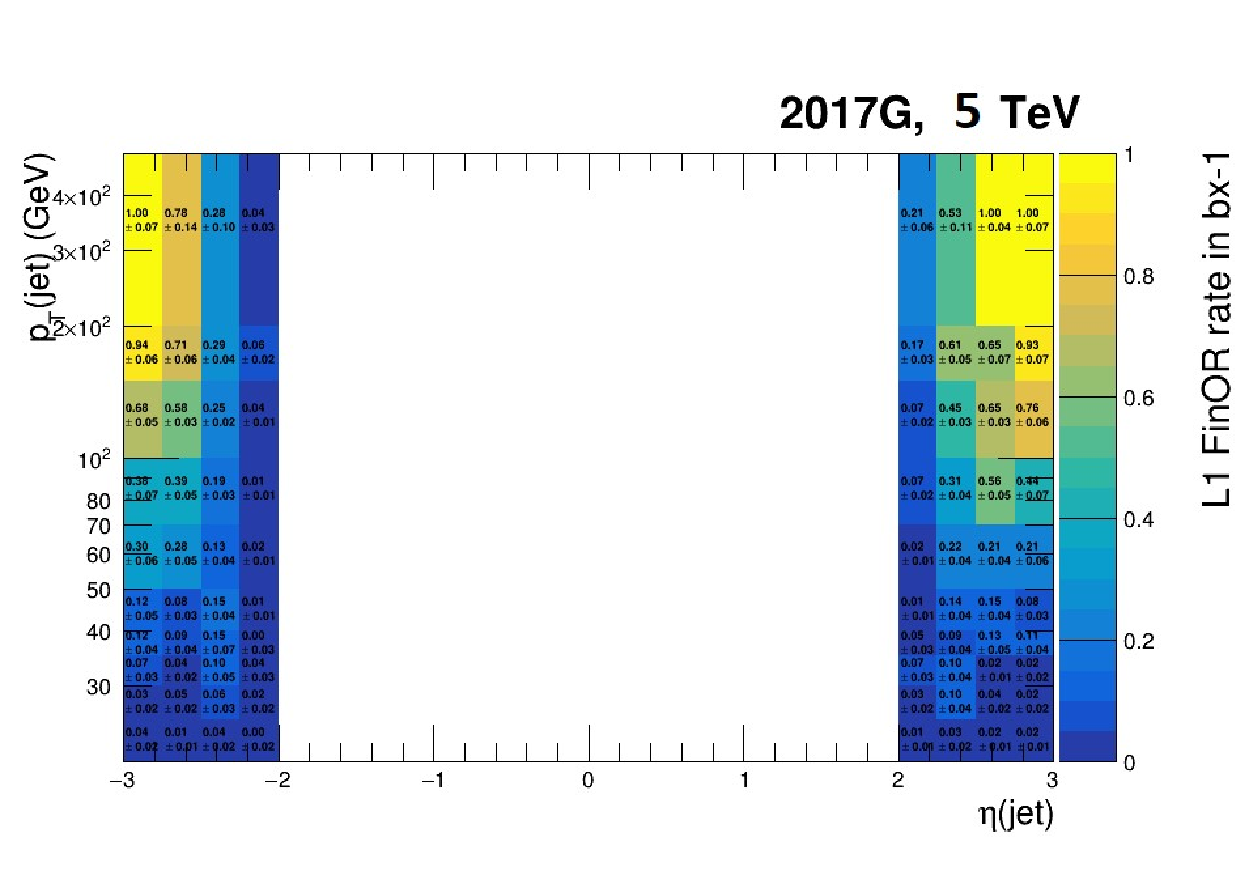
\includegraphics[width=0.49\textwidth]{plots/Prefire/L1prefiring_jetpt_2017G.pdf}
\caption{Pre-firing probability maps for photons (left) and jets (right) for 2017G (\sg). The $z-\mathrm{axis}$ represents the probability of an object with $(\pt,\eta)$ causing pre-firing. Objects with higher \pt and $|\eta| \sim 3$ are more likely to cause pre-firing. Objects with $|\eta| < 2$ do not cause pre-firing.}
\label{fig:prefire:2017G}
\end{figure}

\begin{figure}[htbp]
\centering
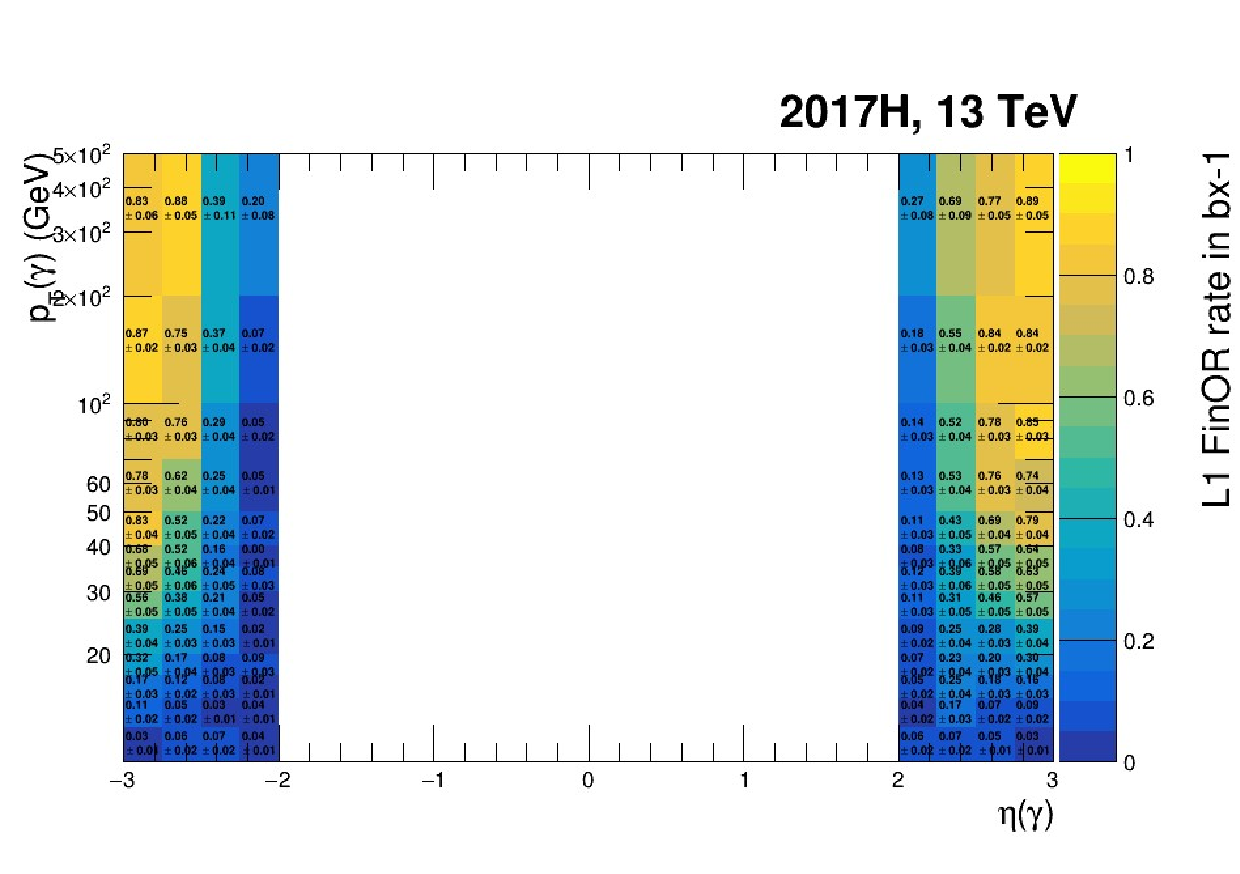
\includegraphics[width=0.49\textwidth]{plots/Prefire/L1prefiring_photonpt_2017H.pdf}
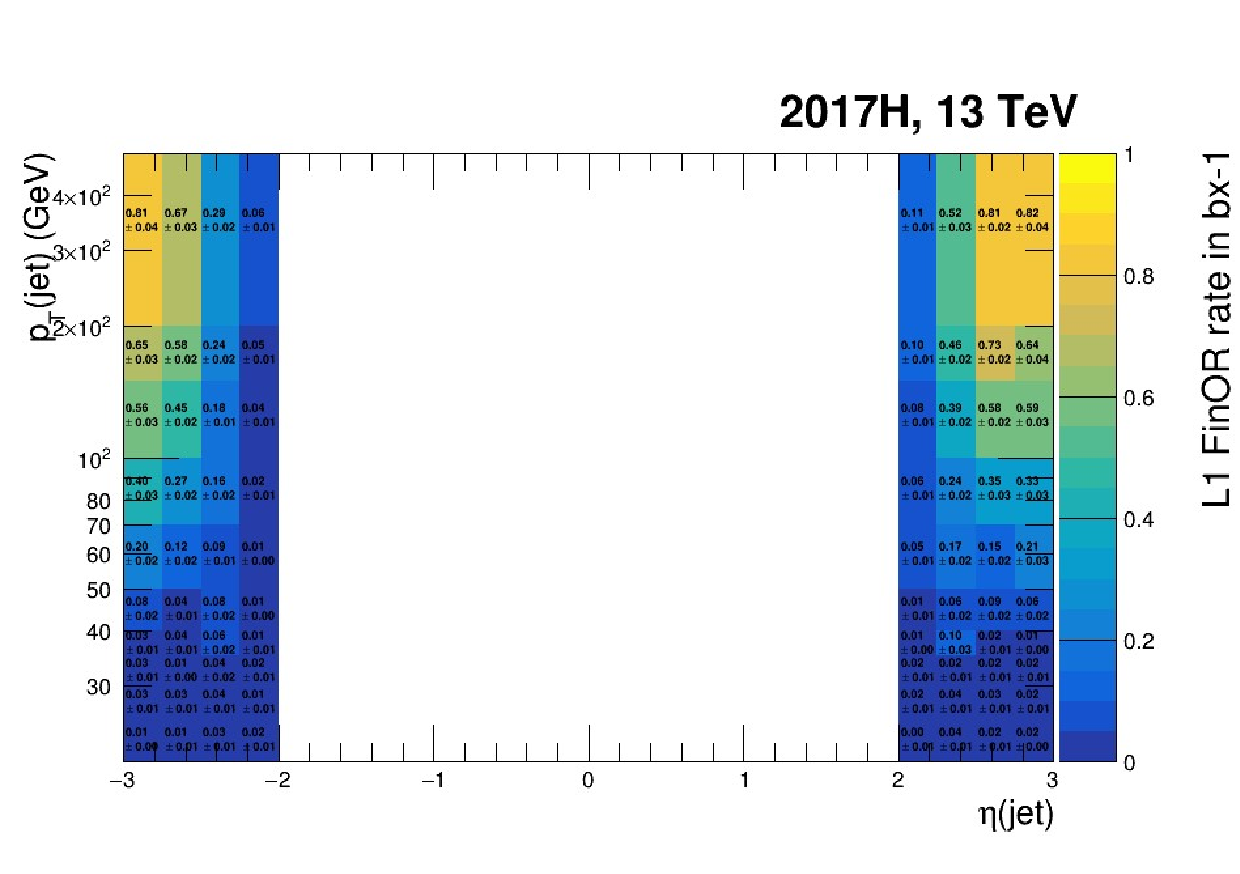
\includegraphics[width=0.49\textwidth]{plots/Prefire/L1prefiring_jetpt_2017H.pdf}
\caption{Pre-firing probability maps for photons (left) and jets (right) for 2017H (\sh). The $z-\mathrm{axis}$ represents the probability of an object with $(\pt,\eta)$ causing pre-firing. Objects with higher \pt and $|\eta| \sim 3$ are more likely to cause pre-firing. Objects with $|\eta| < 2$ do not cause pre-firing.}
\label{fig:prefire:2017H}
\end{figure}
\begin{equation}
    w_{pref} = 1 - P(\mathrm{pre-fire}) = \prod_{i=\gamma,jets}{(1 - \epsilon_i^{pref}(\eta,p_T))}
    \label{eq:prefiring_weight}
\end{equation}
Pre-firing probability maps for jets and photons are shown in Figure~\ref{fig:prefire:2017G} for 2017G (\serag) and Figure~\ref{fig:prefire:2017H} for 2017H (\serah). The probability of pre-firing is derived from a tag-and-probe method requiring a central tag and foward probe to ensure the probe is the source of the pr-efiring. Photon pre-firing prability is derived from the SingleElectron data stream and the jet pre-firing probability is derived from the SingleMuon data stream. In Equation~\ref{eq:prefiring_weight}, the probability of pre-firing due to an individual photon or jet given its \pt and $\eta$ is $\epsilon_i^{pref}(\eta,p_T)$. In events with overlapping photons and jets (with $\Delta  R < 0.4$), only the contribution from the object with the highest probability of pre-firing is used in Equation~\ref{eq:prefiring_weight}\cite{LATHOMAS}. Yield predictions from the \Wpm and \Z boson signal simulation are re-normalized to account for the pre-firing effect, with correction factors listed in Table~\ref{tab:prefire:5} for 2017G (\serag) and Table~\ref{tab:prefire:13} for 2017H (\serah). Uncertainties in the pre-firing probability are 20\%. The effect of pre-firing on the \zee rapidity distribution for 2017G (2017H) is shown in  Figure~\ref{fig:prefire:zrap:2017G} (Figure~\ref{fig:prefire:zrap:2017H}). These figures also demonstrate the effectiveness of the corrections at mitigating the effects of pre-firing on forward events.
\begin{figure}[htb]
\centering
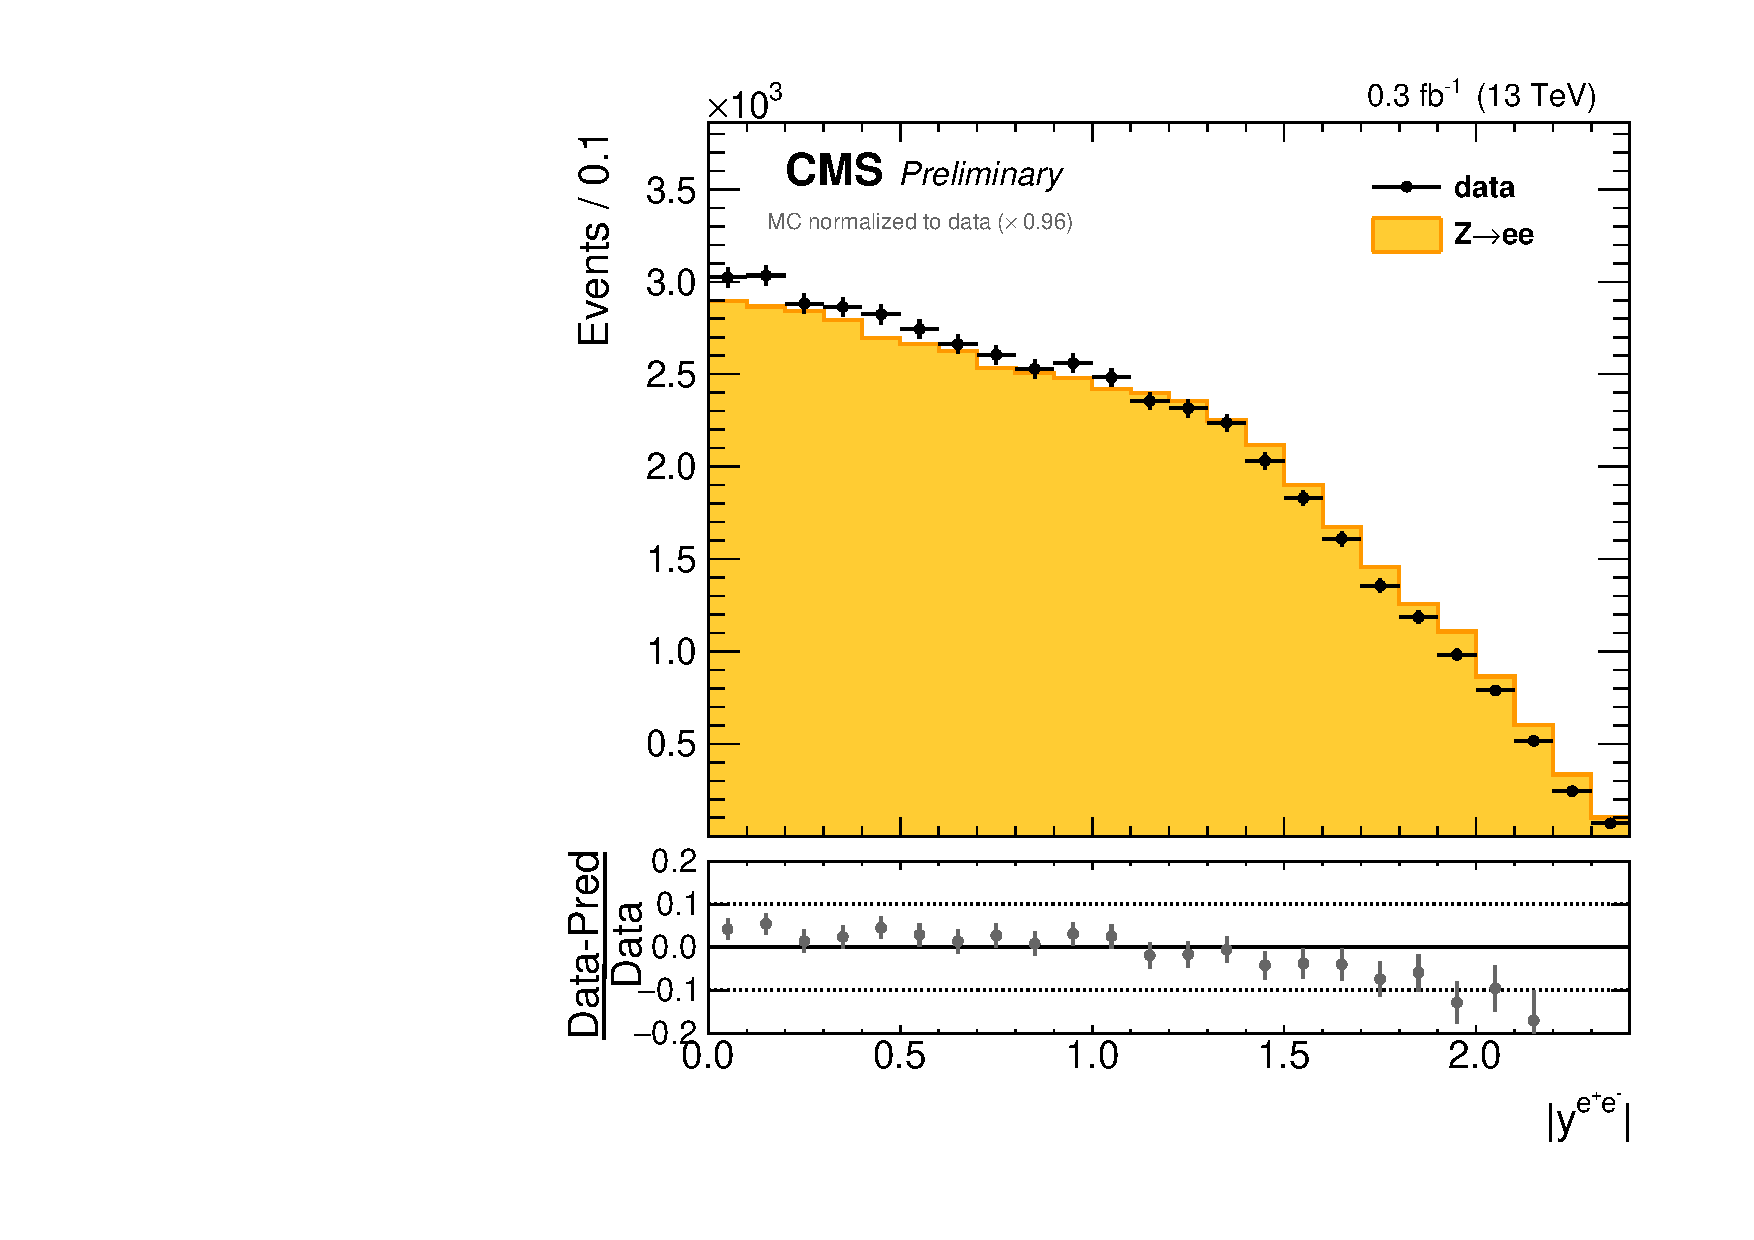
\includegraphics[width=0.49\textwidth]{plots/Prefire/Zee5_Zrap_noPrefire.pdf}
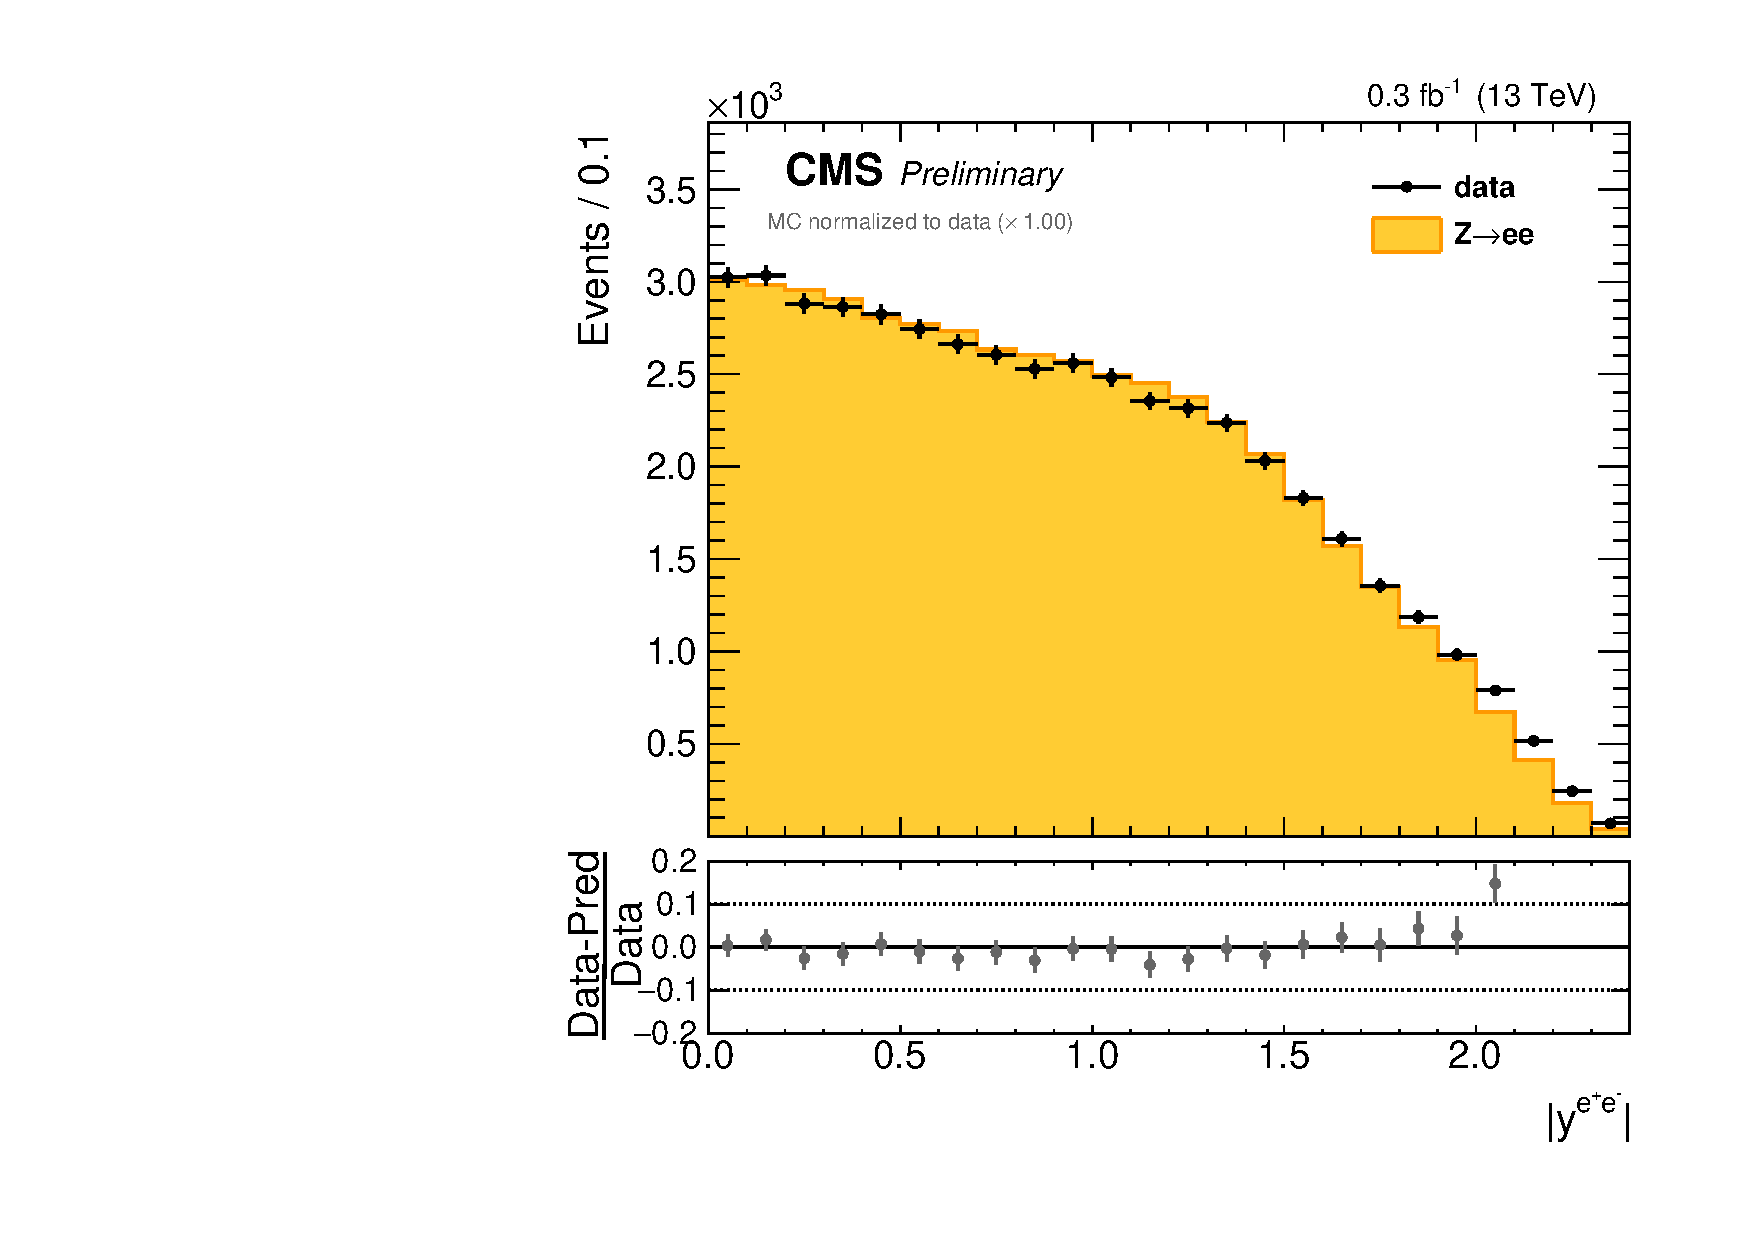
\includegraphics[width=0.49\textwidth]{plots/Prefire/Zee5_Zrap_inclPrefire.pdf}
\caption{\zee rapidity before (left) and after (right) pre-firing corrections, 2017G (\sg).}
\label{fig:prefire:zrap:2017G}
\end{figure}

\begin{figure}[htb]
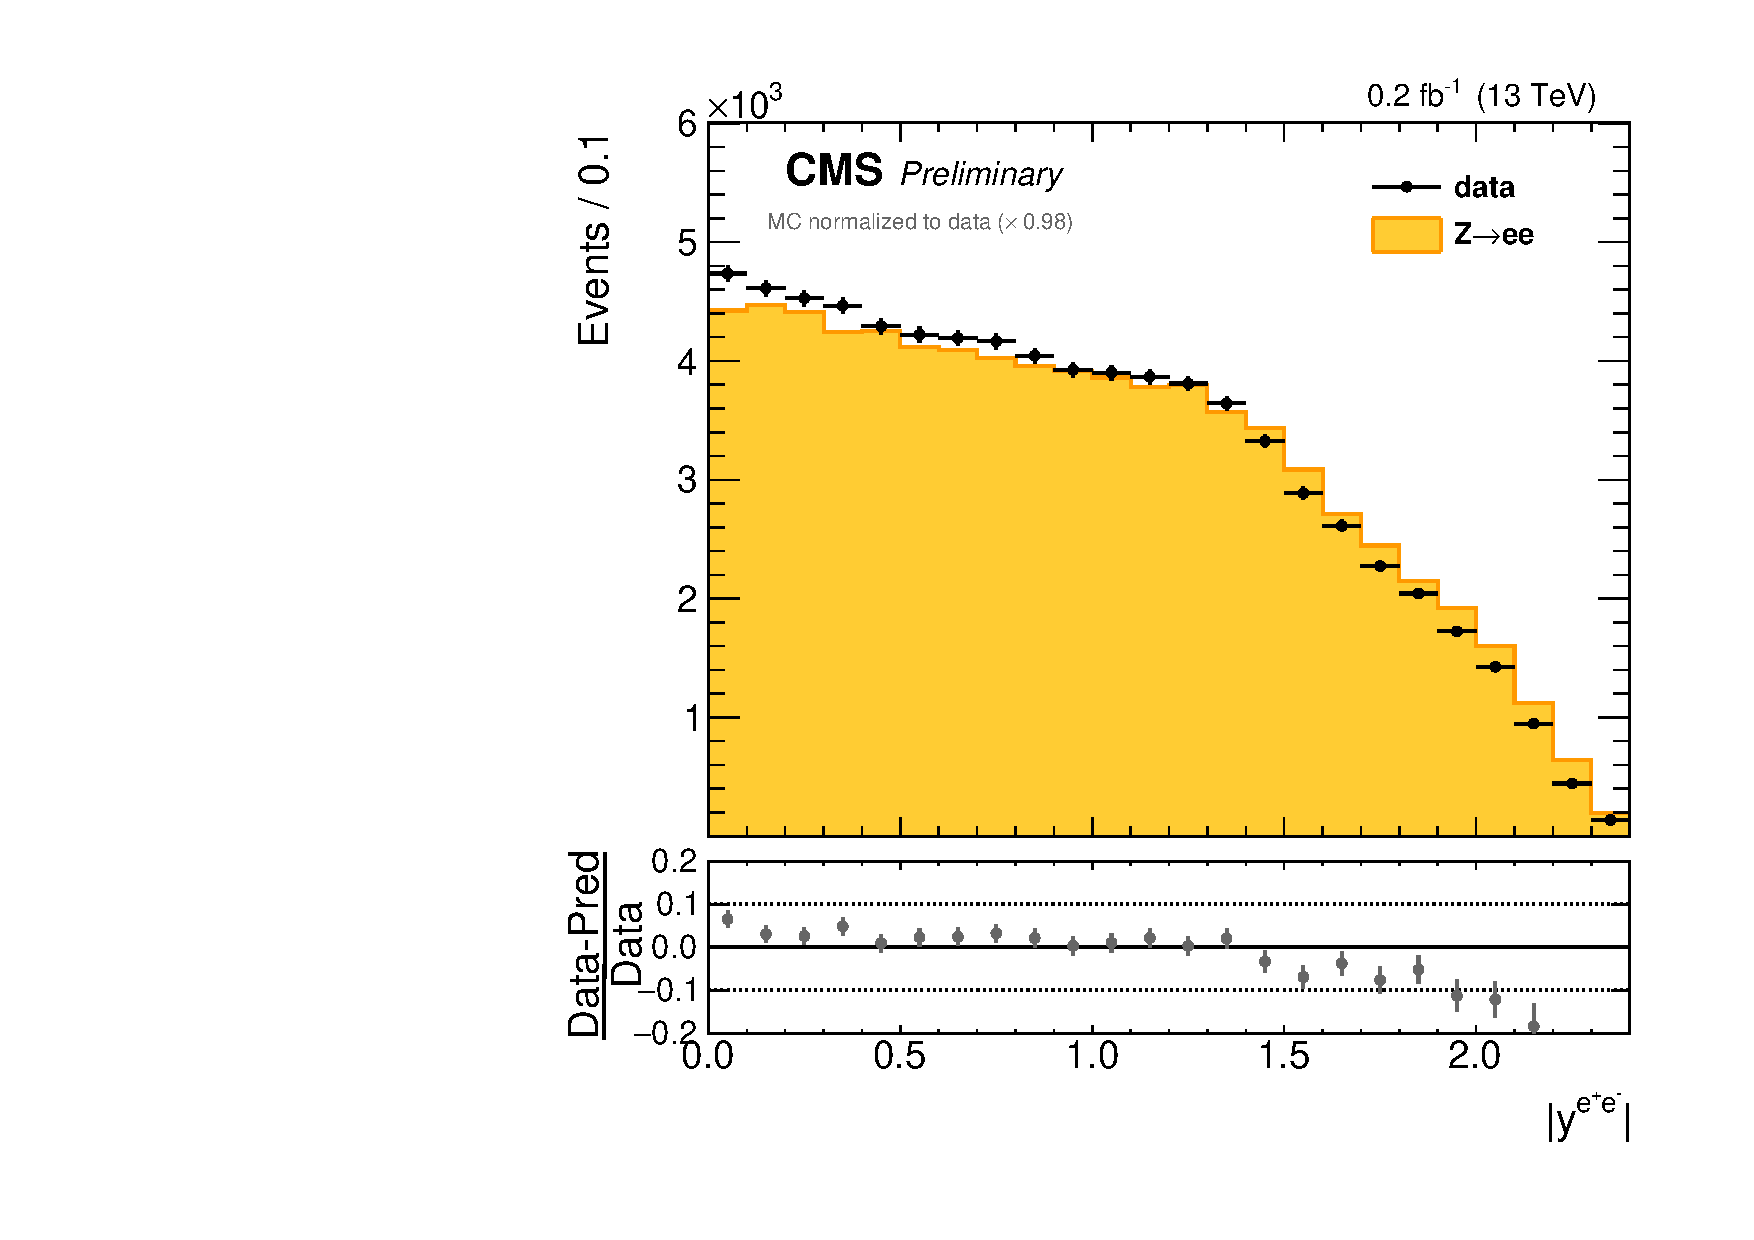
\includegraphics[width=0.49\textwidth]{plots/Prefire/Zee13_Zrap_noPrefire.pdf}
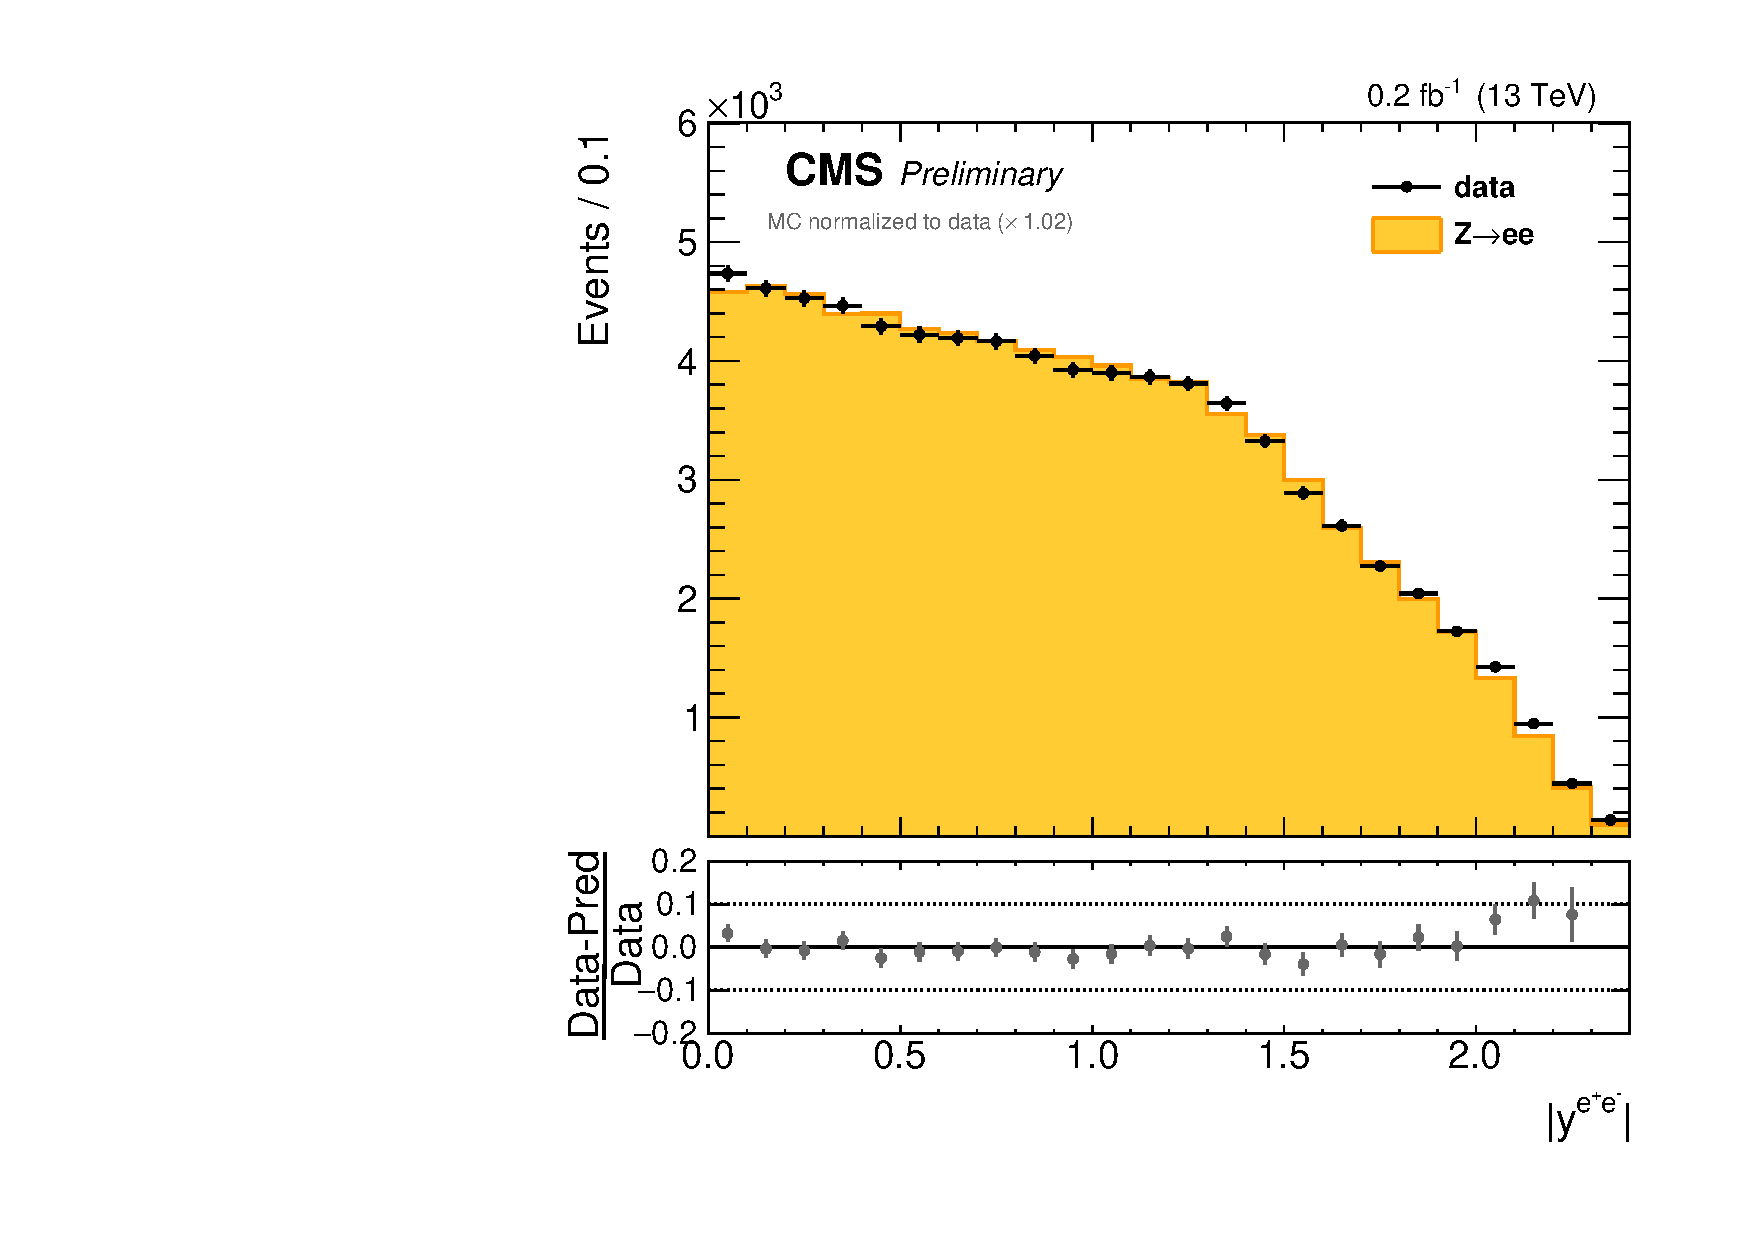
\includegraphics[width=0.49\textwidth]{plots/Prefire/Zee13_Zrap_inclPrefire.pdf}
\caption{\zee rapidity before (left) and after (right) pre-firing corrections, 2017H (\sh).}
\label{fig:prefire:zrap:2017H}
\end{figure}
%%%% Table containing prefire effects, 5 TeV
\begin{table}[htbp]
\begin{center}
\begin{tabular}{|c|c|c|c|c|}
\hline
Process & Jets & Photons & Total \\\hline \hline
$W\rightarrow e^+\nu$      & 0.990 & 0.977 & 0.975 \\
$W\rightarrow e^-\nu$      & 0.990 & 0.978 & 0.976 \\
$Z\rightarrow ee$          & 0.986 & 0.961 & 0.959 \\
\hline
$W\rightarrow \mu^+\nu$   & 0.989 & 0.998 & 0.988 \\
$W\rightarrow \mu^-\nu$   & 0.989 & 0.999 & 0.989\\
$Z\rightarrow \mu\mu$     & 0.985 & 0.999 & 0.985 \\
\hline
\end{tabular} 
\end{center}


\caption{Impact of prefiring on the reconstruction efficiency of each of the \Wp, \Wm, and \Z boson channels for the \sg (2017G) dataset. Corrections are applied differentially and table reports total efficiency integrated over full phase space. The "Total" column includes proper counting of overlapping objects and is the total efficiency scale factor due to pre-firing.}
\label{tab:prefire:5}
\end{table}

%%%% Table containing prefire effects, 13 TeV
\begin{table}[htbp]
\begin{center}
\begin{tabular}{|c|c|c|c|c|}
\hline
Process & Jets & Photons & Total \\\hline \hline
$W\rightarrow e^+\nu$      & 0.989 & 0.970 & 0.967 \\
$W\rightarrow e^-\nu$      & 0.990 & 0.974 & 0.971\\
$Z\rightarrow ee$          & 0.988 & 0.964 & 0.962 \\
\hline
$W\rightarrow \mu^+\nu$   & 0.990 & 0.996 & 0.988 \\
$W\rightarrow \mu^-\nu$   & 0.991 & 0.997 & 0.989 \\
$Z\rightarrow \mu\mu$     & 0.989 & 0.997 & 0.987 \\
\hline
\end{tabular}
\end{center}

\caption{Impact of prefiring on the reconstruction efficiency of each of the \Wp, \Wm, and \Z boson channels for the \sh (2017H) dataset. The "Total" column includes proper counting of overlapping objects and is the scale factor by which the expected number of events is adjusted.}
\label{tab:prefire:13}
\end{table}
